\documentclass[11pt, a4paper]{article}

\usepackage[utf8]{inputenc}
\usepackage[T1]{fontenc}
\usepackage[spanish]{babel}
\usepackage{amsmath, amssymb, amsthm}
\usepackage{geometry}
\usepackage{hyperref}
\usepackage{booktabs}
\usepackage{tabularx}
\usepackage{float}
\usepackage{xcolor}
\usepackage{algorithm}
\usepackage{algpseudocode}
\usepackage{graphicx}

\geometry{margin=2.5cm}

\hypersetup{
  colorlinks=true,
  linkcolor=blue!60!black,
  citecolor=blue!60!black,
  urlcolor=blue!60!black,
}

\theoremstyle{definition}
\newtheorem{definition}{Definición}[section]
\newtheorem{remark}{Observación}[section]
\newtheorem{theorem}{Teorema}[section]
\newtheorem{proposition}{Proposición}[section]
\newtheorem{lemma}{Lema}[section]

\newcommand{\R}{\mathbb{R}}
\newcommand{\E}{\mathbb{E}}
\newcommand{\Prob}{\mathbb{P}}
\newcommand{\norm}[1]{\left\|#1\right\|}
\newcommand{\abs}[1]{\left|#1\right|}
\newcommand{\inner}[2]{\langle #1,\, #2 \rangle}
\newcommand{\eps}{\varepsilon}
\newcommand{\Pdis}{\mathcal{P}}
\newcommand{\dee}{\,\mathrm{d}}

\title{\textbf{Métodos computacionales para Daudin \& Delarue (2025)}\\[0.4em]
\large Aplicación numérica de Neural ODEs de campo medio con regularización entrópica\\
\normalsize Basado en \textit{arXiv:2507.08486}}
\author{Daniel Torres Gonzalez \\ Universidad Complutense de Madrid}
\date{\today}

\begin{document}
\maketitle
\tableofcontents
\newpage

% ============================================================
\section*{Introducción}
\addcontentsline{toc}{section}{Introducción}

Este documento describe en detalle los métodos numéricos implementados para la
aplicación computacional del marco de \textbf{Daudin \& Delarue}~(2025) sobre
\emph{Neural ODEs de campo medio con regularización entrópica}. Cada sección
corresponde a un método distinto de aproximar o calcular la trayectoria
óptima $\boldsymbol{\nu}^* = (\nu_t^*)_{t \in [t_0, T]}$ del control:

\begin{enumerate}
  \item \textbf{Solución explícita} (Sección~\ref{sec:explicita}): aplicación
        directa de la fórmula cerrada del Teorema~1.4 del paper sobre un
        \emph{grid} discreto del espacio de parámetros $A$. Es la
        implementación más fiel posible al marco teórico, sin aproximaciones
        más allá de la discretización espacio-temporal.
  \item \textbf{Regularizadores paramétricos}
        (Sección~\ref{sec:reg-moons}): SGLD vanilla, pSGLD, MMD$^2$ y
        divergencia de Sinkhorn como sustitutos prácticos del término
        entrópico (que es $+\infty$ en la representación por
        $M$-partículas). Comparación sobre \texttt{make\_moons} y, en
        Sección~\ref{sec:regresion-d8}, sobre California Housing en
        $d_1=8$.
  \item \textbf{Bridge interpretativo} (Sección~\ref{sec:bridge}):
        comparación cuantitativa entre la $\nu^*_T$ exacta del solver
        explícito y la nube empírica de neuronas de cada
        regularizador, con MMD$^2$ y los dos primeros momentos como
        métricas.
  \item \textbf{Aplicación económica}
        (Sección~\ref{sec:economia}): replicación del pipeline
        completo (solver explícito + tres proxies + bridge) sobre
        \texttt{ACSIncome}, un dataset demográfico real
        (American Community Survey, California 2018).
  \item \textbf{Trabajo futuro} (Sección~\ref{sec:trabajo-futuro}):
        cuatro líneas naturales que el bridge habilita ---tasas
        cuantitativas de propagación de caos, bridge dinámico,
        regularizador ``DD-aware'', tests de robustez cross-dataset.
\end{enumerate}

% ============================================================
\section{Solución explícita: aplicación directa del Teorema 1.4}
\label{sec:explicita}

% ------------------------------------------------------------
\subsection{Planteamiento del problema}
\label{ssec:planteamiento}

Recordamos el problema de control estudiado en Daudin~\&~Delarue:
\begin{equation}
  \min_{\boldsymbol{\nu}} \;
  J\bigl((t_0, \gamma_0), \boldsymbol{\nu}\bigr)
  \;=\;
  \int_{\R^{d_1} \times \R^{d_2}} L(x, y) \, \dee\gamma_T(x, y)
  \;+\;
  \eps \int_{t_0}^{T}
  \mathcal{E}(\nu_t \,\|\, \nu^{\infty}) \, \dee t,
  \label{eq:Jtotal}
\end{equation}
sujeto a la ecuación de continuidad
\begin{equation}
  \partial_t \gamma_t
  + \mathrm{div}_x \!\left(
    \int_A b(x, a) \, \dee\nu_t(a) \;\gamma_t
  \right) = 0,
  \qquad
  \gamma_{t_0} = \gamma_0.
  \label{eq:cont}
\end{equation}
El control $\boldsymbol{\nu} = (\nu_t)_{t \in [t_0, T]}$ es una trayectoria en
el espacio de medidas de probabilidad sobre el conjunto de parámetros
$A \subset \R^{d'}$. El término entrópico $\mathcal{E}(\nu_t \,\|\, \nu^{\infty})$
es la divergencia de Kullback--Leibler de $\nu_t$ respecto a la medida prior
$\nu^{\infty}(a) \propto \exp(-\ell(a))$, con potencial
\begin{equation}
  \ell(a) = c_1 \abs{a}^4 + c_2 \abs{a}^2,
  \qquad c_1, c_2 > 0
  \label{eq:ell}
\end{equation}
(necesariamente con crecimiento al menos cuártico para garantizar la
desigualdad log-Sobolev y por tanto la condición Polyak--{\L}ojasiewicz, véase
Sec.~1.2 del paper).

\medskip

Para máxima fidelidad al \textbf{Ejemplo~1.3} del paper, fijamos los datos:
\begin{equation}
  d_1 = d_2 = 1,
  \qquad
  L(x, y) = \tfrac{1}{2}(x - y)^2,
  \qquad
  b(x, a) = \sigma(a_1 x + a_2)\, a_0,
  \label{eq:setup}
\end{equation}
con $\sigma = \tanh$ y $a = (a_0, a_1, a_2) \in \R^3$, esto es, $d' = 2 d_1 + 1 = 3$.

\begin{remark}[Por qué $d_1 = d_2 = 1$]
La elección $d_1 = d_2 = 1$ no es estética: las hipótesis del paper
sobre la pérdida cuadrática requieren $d_1 = d_2$, y el grid sobre
$A = \R^{d'}$ con $d' = 2 d_1 + 1$ se vuelve inviable más allá de
$d_1 = 2$. Para $d_1 = 1$: $d' = 3$, grid $10^3$ totalmente manejable.
\end{remark}

% ------------------------------------------------------------
\subsection{Sistema forward--backward y fórmula explícita}
\label{ssec:fb-explicita}

El Teorema~1.4 del paper caracteriza cualquier minimizador
$\boldsymbol{\nu}^* \in \mathcal{A}(t_0)$ del funcional~\eqref{eq:Jtotal}
mediante la fórmula de Gibbs explícita
\begin{equation}
  \boxed{\;
    \nu_t^*(a)
    \;=\;
    \frac{1}{Z_t^*}
    \exp\!\left(
      -\ell(a)
      \;-\;
      \frac{1}{\eps}
      \int_{\R^{d_1} \times \R^{d_2}}
        b(x, a) \cdot \nabla_x u_t^*(x, y)
      \, \dee\gamma_t^*(x, y)
    \right)
  \;}
  \label{eq:nuexpl}
\end{equation}
donde $Z_t^*$ es la constante de normalización, y
$(\boldsymbol{u}^*, \boldsymbol{\gamma}^*)$ resuelven el sistema
forward--backward acoplado:
\begin{equation}
  \begin{cases}
    \displaystyle
    \partial_t \gamma_t^*
    + \mathrm{div}_x\!\bigl( b(x, \nu_t^*) \, \gamma_t^* \bigr) = 0,
    & \gamma_{t_0}^* = \gamma_0,
    \\[1ex]
    \displaystyle
    -\partial_t u_t^*(x, y)
    - b(x, \nu_t^*) \cdot \nabla_x u_t^*(x, y) = 0,
    & u_T^*(x, y) = L(x, y).
  \end{cases}
  \label{eq:fbsystem}
\end{equation}
Aquí hemos abreviado $b(x, \nu_t) := \int_A b(x, a) \, \dee\nu_t(a)$.

\begin{remark}[$\nu^*_t$ identificada con su densidad]
\label{rem:medida-densidad}
La fórmula~\eqref{eq:nuexpl} expresa $\nu^*_t$ por su \emph{densidad}
respecto a la medida de Lebesgue en $A$, no como medida singular. Esto
es legítimo en el setting del Teorema~1.4: bajo las hipótesis del paper
(potencial $\ell$ supercoercivo, $\eps>0$), $\nu^*_t$ es absolutamente
continua respecto a $\nu^\infty$, y por tanto respecto a Lebesgue,
para todo $t\in[t_0,T]$. En el resto del documento usamos
indistintamente la medida y su densidad cuando no hay riesgo de
confusión: $\nu^*_t(a)$ denota el valor puntual de la densidad y
$\int f(a)\,d\nu^*_t(a)$ la integral contra esa misma densidad. La
distinción reaparece sólo al comparar $\nu^*_t$ con sus aproximaciones
\emph{paramétricas} $\tfrac1M\sum_m\delta_{\theta^m(t)}$, que sí son
singulares respecto a Lebesgue (cf.\ Sección~\ref{sec:reg-moons-kl}).
\end{remark}

\medskip

El sistema~\eqref{eq:fbsystem}--\eqref{eq:nuexpl} es de tipo
\emph{Mean-Field Game}: la dinámica forward de las features depende del
control $\nu_t^*$, que a su vez se determina por la dinámica backward
del adjunto $u_t^*$, evaluado contra la misma $\gamma_t^*$. Resolverlo
de forma exacta es generalmente imposible; la idea de nuestra
aproximación es:
\begin{enumerate}
  \item Discretizar el espacio $A$ en un \emph{grid} finito
        $\{a^l\}_{l=1}^{M}$ para que $\nu_t^*$ se reduzca a un vector
        de probabilidades $\{\nu_t^*(a^l)\}_{l=1}^{M}$.
  \item Discretizar $\gamma_t^*$ por $N$ partículas $(X_i(t), y_i)$.
  \item Resolver~\eqref{eq:fbsystem}--\eqref{eq:nuexpl} por una iteración
        de tipo Picard (punto fijo).
  \item Calcular el adjunto $u^*$ por el método de las características,
        evitando integrar la EDP backward explícitamente.
\end{enumerate}

% ------------------------------------------------------------
\subsection{Aproximar $\nu_t$}
\label{ssec:neural-interp}

\paragraph{Las dos formas de aproximar $\nu_t$.}
En la práctica $\nu_t$ no se representa exactamente; se aproxima de
una de dos maneras complementarias:

\begin{itemize}
  \item \textbf{Aproximación \emph{paramétrica} con $M$ partículas
        (Tareas~2 y~3, Sec.~\ref{sec:reg-moons} y posteriores).}
        Se fijan $M$ neuronas
        $\{\theta^m\}_{m=1}^{M} \subset A$ y se identifica
        $\nu_t \approx \tfrac{1}{M}\sum_{m=1}^{M} \delta_{\theta^m(t)}$.
        \textbf{Las posiciones $\theta^m$ se aprenden} (descenso por
        gradiente, pSGLD\ldots) y se mueven libremente por $A$. La red
        es la familiar \texttt{MeanFieldResNet}: ``$M$ neuronas con
        parámetros entrenables''.

  \item \textbf{Aproximación \emph{explícita} sobre un grid
        (esta sección).}
        Se fijan $M$ neuronas \emph{candidatas} $\{a^l\}_{l=1}^{M}$
        en posiciones \emph{predeterminadas} (puntos de un grid
        regular sobre $A$) y se identifica
        $\nu_t \approx \sum_{l=1}^{M} \nu_t(a^l)\,\delta_{a^l}$.
        \textbf{Las posiciones $a^l$ no se mueven}; lo único que se
        optimiza es el \emph{vector de probabilidades}
        $(\nu_t(a^l))_{l=1}^M$ que dice ``cuánto pesa cada neurona
        del catálogo en el tiempo $t$''.
\end{itemize}

\paragraph{Por qué el grid en este enfoque.}
La fórmula del Teorema~1.4
(ec.~\ref{eq:nuexpl}) caracteriza $\nu_t^*$ como una distribución
de Gibbs:
\[
  \nu_t^*(a) \;\propto\; \exp\!\Bigl(-\ell(a) - \tfrac{1}{\eps}
  \mathbb E_{\gamma_t^*}\!\bigl[b(x, a)\!\cdot\!\nabla_x u_t^*\bigr]\Bigr).
\]
Para \emph{evaluar} esta densidad y para \emph{normalizarla}
($\int_A \nu_t^* = 1$) hacen falta integrales sobre $A$. El grid es
la herramienta más simple para hacerlas: se reemplaza
$\int_A \nu_t^*(a)\, da$ por una suma sobre los puntos del grid y
$\nu_t^*$ pasa a ser un \emph{vector de longitud $M$}, manejable y
diferenciable.

\paragraph{Limitaciones del grid.}
El grid uniforme escala como $M = M_{\mathrm{pd}}^{2 d_1 + 1}$
puntos por dimensión. Para $d_1 = 1$ ($A = \mathbb R^3$) basta
$M_{\mathrm{pd}} = 10$ y $M = 1\,000$; para $d_1 = 8$
($A = \mathbb R^{17}$) ya con $M_{\mathrm{pd}} = 3$ se llegaría a
$3^{17} \approx 1{,}3 \cdot 10^8$ puntos: \emph{maldición de la
dimensionalidad}. Por eso el enfoque explícito (esta sección) sólo
es viable en dimensión baja, mientras que la aproximación
paramétrica con $M$ partículas (siguientes secciones) escala bien.

% ------------------------------------------------------------
\subsection{Discretizaciones}
\label{ssec:discret}

\subsubsection{Discretización del espacio de parámetros $A$}

Construimos un grid uniforme cartesiano sobre $[-R, R]^3 \subset A$:
\begin{equation}
  \{a^l\}_{l=1}^{M} \;:=\; \left\{
  \bigl( g_{i_0},\, g_{i_1},\, g_{i_2} \bigr)
  \;:\; i_0, i_1, i_2 \in \{1, \dots, M_{\mathrm{dim}}\}
  \right\},
  \quad
  g_i = -R + \tfrac{2R\,(i-1)}{M_{\mathrm{dim}} - 1},
\end{equation}
con $M = M_{\mathrm{dim}}^3$ puntos. En todos los experimentos usamos
$R = 2.5$ y $M_{\mathrm{dim}} = 10$, es decir, $M = 1000$.

\medskip

La medida prior $\nu^{\infty}$, restringida al grid y normalizada, es
\begin{equation}
  \nu^{\infty}(a^l)
  \;=\;
  \frac{\exp(-\ell(a^l))}{\sum_{l'=1}^{M} \exp(-\ell(a^{l'}))}.
  \label{eq:nuinfgrid}
\end{equation}
La elección $R = 2.5$ cubre más del $99\%$ de la masa de la prior continua,
ya que $\ell(a) \geq c_1 \abs{a}^4$ decae rápidamente fuera de la bola
unidad.

\subsubsection{Discretización temporal}

Particionamos $[t_0, T] = [0, T]$ en $K$ subintervalos de tamaño
$\Delta t = T/K$:
\begin{equation}
  t_k = k \, \Delta t, \quad k = 0, 1, \dots, K.
\end{equation}
La trayectoria de la medida $\nu_t^*$ se almacena como una matriz
$\boldsymbol{\nu} \in \R^{(K+1) \times M}$ con
$\boldsymbol{\nu}_{k, l} \approx \nu_{t_k}^*(a^l)$.

\subsubsection{Discretización de $\gamma_t^*$ por partículas}

Sustituimos la medida $\gamma_t$ por la suma empírica sobre $N$
partículas con etiquetas fijas:
\begin{equation}
  \gamma_t^{(N)} = \frac{1}{N} \sum_{i=1}^{N}
    \delta_{(X_i(t),\, y_i)},
  \quad
  X_i(0) = x_i,
  \;\;
  i = 1, \dots, N.
  \label{eq:gammaN}
\end{equation}
Cada partícula evoluciona según la ODE
\begin{equation}
  \dot{X}_i(t)
  \;=\;
  \int_A b(X_i(t), a) \, \dee\nu_t(a)
  \;\approx\;
  \sum_{l=1}^{M} b(X_i(t), a^l) \, \nu_{t}(a^l).
  \label{eq:Xdot}
\end{equation}

% ------------------------------------------------------------
\subsection{Backward por el método de las características}
\label{ssec:caracteristicas}

La ecuación backward del sistema~\eqref{eq:fbsystem},
\begin{equation}
  -\partial_t u_t - b(x, \nu_t) \cdot \nabla_x u_t = 0,
  \qquad u_T = L,
\end{equation}
es una \emph{ecuación de transporte} cuyas características son
exactamente las trayectorias de la dinámica forward. Esto permite
obtener $u^*$ \emph{sin integrar la EDP}, simplemente leyendo $L$ al
tiempo final a lo largo del flujo:
\begin{equation}
  u_t^*(x, y)
  \;=\;
  L\bigl( X^{t, x}(T),\, y \bigr),
  \label{eq:ucharac}
\end{equation}
donde $X^{t, x}(s)$ denota la solución de~\eqref{eq:Xdot} en tiempo $s$
con condición inicial $x$ en tiempo $t$.

\medskip

\textbf{Gradiente espacial $\nabla_x u_t^*$.} Para evaluar la
fórmula~\eqref{eq:nuexpl} necesitamos
$\nabla_x u_t^*(X_i(t), y_i)$. Por la regla de la cadena
aplicada a~\eqref{eq:ucharac}, con $L(x, y) = \tfrac{1}{2}(x - y)^2$:
\begin{equation}
  \nabla_x u_t^*(x, y)
  \;=\;
  \bigl( X^{t, x}(T) - y \bigr)
  \cdot
  \frac{\partial X^{t, x}(T)}{\partial x}.
  \label{eq:nablau}
\end{equation}

\textbf{Sensibilidad de la trayectoria.} Para cada partícula $i$,
denotemos
\begin{equation}
  \Phi_i(t) \;:=\; \frac{\partial X_i(t)}{\partial X_i(0)},
\end{equation}
es decir, la sensibilidad de la trayectoria respecto a su condición
inicial (usamos la letra $\Phi$, habitual para la \emph{matriz
fundamental} en EDOs lineales, para no colisionar con el funcional de
coste $J$ de~\eqref{eq:Jtotal}). Esta función satisface la
\emph{ecuación variacional}:
\begin{equation}
  \dot{\Phi}_i(t)
  \;=\;
  \frac{\partial}{\partial x}
  \!\left[
    \int_A b(X_i(t), a) \, \dee\nu_t(a)
  \right]_{x = X_i(t)}
  \cdot \Phi_i(t),
  \qquad
  \Phi_i(0) = 1.
  \label{eq:Jdot}
\end{equation}
En el caso $d_1 = 1$, $\Phi_i(t)$ es \emph{escalar}, lo que simplifica
mucho la implementación. Por la propiedad del cociclo del flujo:
\begin{equation}
  \frac{\partial X^{t, X_i(t)}(T)}{\partial x}
  \;=\;
  \frac{\Phi_i(T)}{\Phi_i(t)}.
\end{equation}
Así, sustituyendo en~\eqref{eq:nablau} con $x = X_i(t)$,
$y = y_i$, obtenemos la fórmula computable:
\begin{equation}
  \boxed{\;
    \nabla_x u_t^*\bigl( X_i(t),\, y_i \bigr)
    \;=\;
    \bigl( X_i(T) - y_i \bigr) \cdot \frac{\Phi_i(T)}{\Phi_i(t)}.
  \;}
  \label{eq:nablau-final}
\end{equation}
Esta identidad es la pieza clave que evita resolver la EDP backward
por diferencias finitas o por método adjunto: basta integrar
\emph{conjuntamente} $(X_i, \Phi_i)$ por~\eqref{eq:Xdot} y~\eqref{eq:Jdot}
durante el paso forward y, al terminar, leer~\eqref{eq:nablau-final}
en cualquier $t_k$ deseado.

% ------------------------------------------------------------
\subsection{Aproximación de la fórmula explícita en el grid}
\label{ssec:gibbsdiscret}

Sustituyendo la aproximación empírica
$\gamma_t^* \approx \gamma_t^{(N)}$ y la
identidad~\eqref{eq:nablau-final} en~\eqref{eq:nuexpl}, obtenemos la
versión discretizada de la fórmula de Gibbs sobre el grid:
\begin{equation}
  \log \nu_{t_k}^*(a^l)
  \;=\;
  -\ell(a^l)
  \;-\;
  \frac{1}{\eps N}
  \sum_{i=1}^{N}
    b\bigl( X_i(t_k), a^l \bigr)
    \cdot
    \bigl( X_i(T) - y_i \bigr) \,
    \frac{\Phi_i(T)}{\Phi_i(t_k)}
  \;-\;
  \log Z_{t_k}^{(M)},
  \label{eq:nuexpl-discret}
\end{equation}
con $Z_{t_k}^{(M)}$ la constante de normalización en el grid. Numéricamente
calculamos el lado derecho con \texttt{logsumexp} para evitar
\texttt{overflow}.

% ------------------------------------------------------------
\subsection{Coste discreto}
\label{ssec:coste}

El funcional~\eqref{eq:Jtotal}, evaluado sobre las discretizaciones,
se escribe
\begin{equation}
  J^{(N, M, K)}(\boldsymbol{\nu})
  \;=\;
  \underbrace{\frac{1}{N} \sum_{i=1}^{N} \tfrac{1}{2}\bigl( X_i(T) - y_i \bigr)^2}_{\text{término terminal}}
  \;+\;
  \eps \, \Delta t \,
  \underbrace{\sum_{k=0}^{K} \mathrm{KL}\bigl( \boldsymbol{\nu}_k \,\|\, \nu^{\infty} \bigr)}_{\text{término entrópico}},
\end{equation}
donde la KL discreta es
\begin{equation}
  \mathrm{KL}(\boldsymbol{\nu}_k \,\|\, \nu^{\infty})
  \;=\;
  \sum_{l=1}^{M} \boldsymbol{\nu}_{k, l}
  \,\log\!\frac{\boldsymbol{\nu}_{k, l}}{\nu^{\infty}(a^l)},
\end{equation}
con la convención usual $0 \log 0 = 0$.

\begin{remark}[KL finita]
Una de las motivaciones principales de la discretización por grid es
que la divergencia $\mathrm{KL}(\nu_{t_k} \,\|\, \nu^{\infty})$ es
\emph{finita}: ambas medidas son discretas sobre el mismo soporte
finito $\{a^l\}$. En contraste, las aproximaciones por partículas
$\nu_t^{(M)} = \tfrac{1}{M}\sum_m \delta_{a^m}$ producen
$\mathrm{KL}(\nu_t^{(M)} \,\|\, \nu^{\infty}) = +\infty$ porque
$\nu_t^{(M)}$ es discreta y $\nu^{\infty}$ continua. Esta es la
limitación que motiva los métodos sustitutivos (pSGLD, MMD, Sinkhorn)
de las secciones siguientes.
\end{remark}

% ------------------------------------------------------------
\subsection{Algoritmo: iteración de Picard con punto fijo}
\label{ssec:picard}

El sistema~\eqref{eq:fbsystem}--\eqref{eq:nuexpl} es un \emph{problema
de punto fijo}: $\nu_t^*$ depende de $(\gamma_t^*, u_t^*)$, que a su vez
dependen de $\nu_t^*$. Iteramos:

\begin{algorithm}[H]
\caption{Picard fixed-point para la solución explícita}
\label{alg:picard}
\begin{algorithmic}[1]
\State \textbf{Entrada:} dataset $\{(x_i, y_i)\}_{i=1}^{N}$, grid
       $\{a^l\}_{l=1}^{M}$, hiperparámetros
       $T, K, \eps, c_1, c_2$, factor de damping $\omega \in (0, 1]$,
       tolerancia $\tau$, $\nu_{\mathrm{init}}$ opcional.
\State Calcular $\nu^{\infty}(a^l)$ por~\eqref{eq:nuinfgrid}.
\State Inicializar $\boldsymbol{\nu}^{(0)}_{k} \leftarrow \nu^{\infty}$ para todo $k$
       (o $\nu_{\mathrm{init}}$ si se proporciona).
\For{$j = 0, 1, 2, \dots$ hasta $\max_k \norm{\boldsymbol{\nu}^{(j+1)}_k - \boldsymbol{\nu}^{(j)}_k}_{\mathrm{TV}}/2 < \tau$}
  \State \textbf{Forward:} integrar $(X_i, \Phi_i)$ por RK4 sobre $[0, T]$ con
         control $\boldsymbol{\nu}^{(j)}$, usando~\eqref{eq:Xdot}
         y~\eqref{eq:Jdot}.
  \State \textbf{Update Gibbs:} para cada $k = 0, \dots, K$ y cada
         $l = 1, \dots, M$, calcular
         $\tilde{\boldsymbol{\nu}}_{k, l}$
         por~\eqref{eq:nuexpl-discret} usando
         $X_i(t_k)$, $\Phi_i(t_k)$, $\Phi_i(T)$, $X_i(T)$.
  \State \textbf{Damping:}
         $\boldsymbol{\nu}^{(j+1)}_{k} \leftarrow
          (1 - \omega)\, \boldsymbol{\nu}^{(j)}_{k}
          + \omega\, \tilde{\boldsymbol{\nu}}_{k}$,
         renormalizando.
\EndFor
\State \textbf{Salida:} $\boldsymbol{\nu}^{(j)}$ (ley óptima discreta),
       $\{X_i(t_k)\}_{i, k}$ (trayectorias),
       $\{\Phi_i(t_k)\}_{i, k}$ (Jacobianos del flujo),
       y $J^{(N, M, K)}(\boldsymbol{\nu}^{(j)})$ (coste discreto evaluado en
       la última iteración).
\end{algorithmic}
\end{algorithm}

\begin{remark}[Damping]
El factor $\omega \in (0, 1]$ es necesario para estabilidad. Sin
damping ($\omega = 1$), Picard puede oscilar entre dos puntos lejanos
del óptimo, especialmente cuando $\eps$ es pequeño y la fórmula de
Gibbs produce concentraciones agresivas. Empíricamente $\omega = 0.2\text{--}0.3$
funciona bien para el rango de $\eps$ explorado.
\end{remark}

\begin{remark}[Integrador RK4 con $\nu$ interpolada]
El paso RK4 estándar evalúa el campo en cuatro instantes intermedios
del subintervalo $[t_k, t_{k+1}]$. Como $\nu_t$ está discretizada
sólo en los nodos $t_k$, interpolamos linealmente entre
$\boldsymbol{\nu}_k$ y $\boldsymbol{\nu}_{k+1}$ para los sub-pasos
intermedios. Esta es una decisión de implementación, no del paper.
\end{remark}

% ------------------------------------------------------------
\subsection{Continuación en $\eps$ (warm-start)}
\label{ssec:continuacion}

Para valores pequeños de $\eps$, la fórmula de
Gibbs~\eqref{eq:nuexpl-discret} concentra mucha masa en pocos puntos
del grid, y Picard \emph{frío} (inicializado en $\nu^{\infty}$) cicla
sin converger. Implementamos una estrategia de \emph{continuación} que
calienta progresivamente el problema:

\begin{algorithm}[H]
\caption{Continuación en $\eps$}
\label{alg:continuacion}
\begin{algorithmic}[1]
\State \textbf{Entrada:} secuencia decreciente
       $\eps_1 > \eps_2 > \dots > \eps_S$.
\State $\boldsymbol{\nu}_{\mathrm{warm}} \leftarrow \nu^{\infty}$.
\For{$s = 1, 2, \dots, S$}
  \State Resolver Picard (Algoritmo~\ref{alg:picard}) con
         $\eps = \eps_s$ y
         $\nu_{\mathrm{init}} = \boldsymbol{\nu}_{\mathrm{warm}}$.
  \State $\boldsymbol{\nu}_{\mathrm{warm}} \leftarrow $ solución
         devuelta por Picard.
\EndFor
\end{algorithmic}
\end{algorithm}

Empíricamente, esta estrategia extiende el rango estable de $\eps$ desde
$\eps \geq 0.05$ (frío) hasta $\eps \geq 0.02$ (con continuación) en
los datasets considerados.

% ------------------------------------------------------------
\subsection{Experimentos}
\label{ssec:exp-explicita}

\subsubsection{Configuración común}

\begin{table}[H]
\centering
\begin{tabular}{ll}
\toprule
Hiperparámetro & Valor \\
\midrule
Dimensiones & $d_1 = d_2 = 1$, $d' = 3$ \\
Pérdida & $L(x, y) = \tfrac{1}{2}(x - y)^2$ \\
Activación & $\sigma = \tanh$ \\
Potencial & $\ell(a) = c_1 \abs{a}^4 + c_2 \abs{a}^2$, $(c_1, c_2) = (0.05,\, 0.5)$ \\
Grid & $[-2.5,\, 2.5]^3$, $M_{\mathrm{dim}} = 10 \Rightarrow M = 1000$ \\
Horizonte & $T = 1$, $K = 20$, $\Delta t = 0.05$ \\
Integrador & RK4 con $\nu$ interpolada linealmente \\
Damping & $\omega = 0.2\text{--}0.3$ \\
Tolerancia & $\tau = 10^{-5}$ en $\norm{\cdot}_{\mathrm{TV}}$ \\
Continuación & $\eps \in \{0.5,\, 0.2,\, 0.1,\, 0.05,\, 0.02\}$ \\
\bottomrule
\end{tabular}
\caption{Configuración por defecto del solver explícito.}
\label{tab:setup}
\end{table}

\subsubsection{Datasets}

Usamos dos datasets reales 1D$\to$1D, ambos cargados de
\texttt{vincentarelbundock.github.io/Rdatasets}:

\begin{itemize}
  \item \textbf{Old Faithful} (\texttt{faithful.csv}): $N = 272$
    observaciones del géiser de Yellowstone, con $x = $ duración de la
    erupción e $y = $ tiempo de espera hasta la siguiente. Correlación
    $\rho \approx 0.90$, relación esencialmente lineal.
  \item \textbf{trees} (\texttt{trees.csv}): $N = 31$ árboles de cerezo,
    con $x = $ \emph{Girth} (diámetro del tronco) e $y = $ \emph{Volume}
    (volumen de madera). Correlación $\rho \approx 0.97$, relación
    \emph{no lineal} de tipo $V \propto G^2$ (ley geométrica del cilindro).
\end{itemize}
Las features y etiquetas se estandarizan independientemente
($\mu = 0$, $\sigma = 1$) antes del entrenamiento.

Como referencia teórica, comparamos contra el ajuste OLS lineal sin
intercepto (válido tras estandarizar):
\begin{equation}
  \hat{a}_{\mathrm{OLS}}
  \;=\;
  \frac{\sum_i x_i y_i}{\sum_i x_i^2},
  \qquad
  \mathrm{MSE}/2 \;=\;
  \frac{1}{2N} \sum_i (\hat{a}_{\mathrm{OLS}} x_i - y_i)^2.
\end{equation}
Esta es la \emph{cota inferior} para problemas con relación
exclusivamente lineal y \emph{cota superior alcanzable} cuando la
mean-field ResNet sólo recupera la dependencia lineal.

\subsubsection{Resultados}

\begin{table}[H]
\centering
\begin{tabular}{lrrrrr}
\toprule
$\eps$ & iter. & convergido & $J$ & término L & disp. media \\
\midrule
\multicolumn{6}{l}{\textit{Old Faithful} (OLS lineal: $\mathrm{MSE}/2 = 0.0943$)} \\
\midrule
$0.500$ & 23 & sí & $0.0983$ & $0.0976$ & $0.017$ \\
$0.200$ & 22 & sí & $0.0975$ & $0.0964$ & $0.032$ \\
$0.100$ & 23 & sí & $0.0967$ & $0.0954$ & $0.046$ \\
$0.050$ & 26 & sí & $0.0959$ & $0.0946$ & $0.060$ \\
$0.020$ & 29 & sí & $0.0948$ & $\mathbf{0.0936}$ & $0.074$ \\
\midrule
\multicolumn{6}{l}{\textit{trees} (OLS lineal: $\mathrm{MSE}/2 = 0.0323$)} \\
\midrule
$0.500$ & 23 & sí & $0.0326$ & $0.0323$ & $0.007$ \\
$0.200$ & 24 & sí & $0.0323$ & $0.0318$ & $0.015$ \\
$0.100$ & 26 & sí & $0.0319$ & $0.0312$ & $0.022$ \\
$0.050$ & 28 & sí & $0.0314$ & $0.0304$ & $0.031$ \\
$0.020$ & 30 & sí & $0.0303$ & $\mathbf{0.0285}$ & $0.042$ \\
\bottomrule
\end{tabular}
\caption{Resultados de la solución explícita por continuación en
$\eps$. ``Disp. media'' es $\frac{1}{N}\sum_i \abs{X_i(T) - X_i(0)}$,
una medida del trabajo realizado por el flujo.}
\label{tab:resultados}
\end{table}

\textbf{Lectura.}
\begin{itemize}
  \item En \textbf{Old Faithful}, el término $L$ converge a
        $0.0936$, ligeramente \emph{por debajo} de OLS ($0.0943$).
        El gap es marginal: el dataset es esencialmente lineal,
        y la mean-field ResNet sólo puede aprovechar muy poca
        no linealidad.
  \item En \textbf{trees}, el término $L$ desciende hasta $0.0285$
        (un $12\%$ por debajo de OLS = $0.0323$). Esto demuestra
        que la mean-field ResNet \emph{captura} la no linealidad
        $V \propto G^2$.
  \item En ambos casos, la desviación entre el coste total $J$ y el
        término $L$ corresponde exactamente al término entrópico
        $\eps \, \Delta t \sum_k \mathrm{KL}$, como debe ser por
        construcción.
\end{itemize}

\begin{figure}[H]
\centering
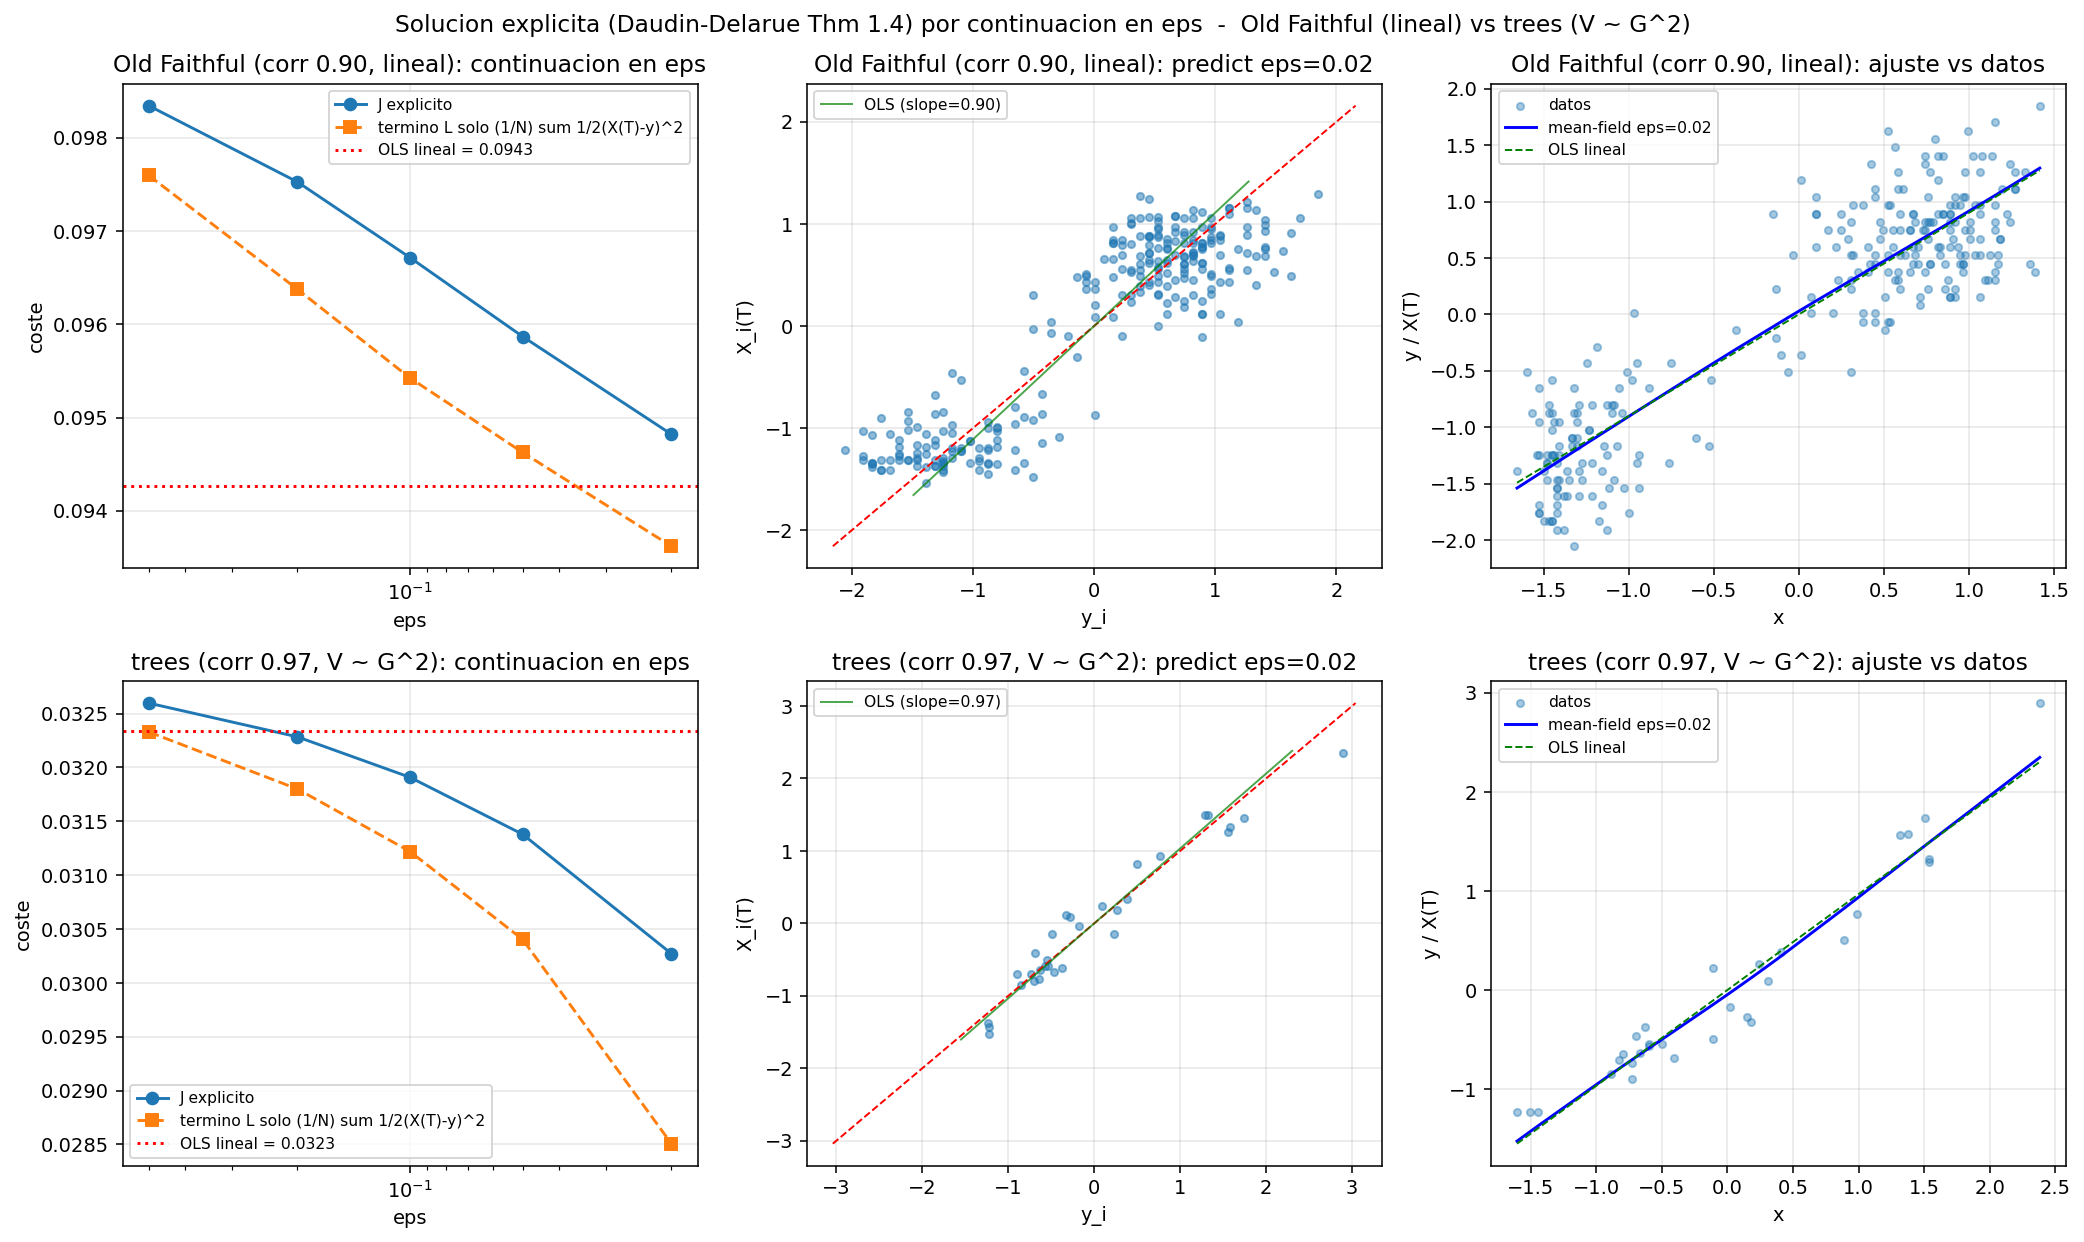
\includegraphics[width=\textwidth]{../figures/01_continuation_faithful_vs_trees.png}
\caption{Solución explícita por continuación en $\eps$. \emph{Fila
superior:} Old Faithful (lineal). \emph{Fila inferior:} trees
($V \propto G^2$). \emph{Columna 1:} cost vs $\eps$. \emph{Columna 2:}
predicciones $X_i(T)$ contra $y_i$ para el menor $\eps$ convergido.
\emph{Columna 3:} ajuste mean-field (azul) sobre los datos crudos
junto con el OLS lineal (verde discontinuo); en \emph{trees} se
observa la curvatura.}
\label{fig:explicita}
\end{figure}

% ------------------------------------------------------------
\subsection{Alternativas numéricas para subir el techo dimensional}
\label{ssec:alternativas-numericas}

El cuello de botella del solver explícito es la cuadratura del grid
tensorial: $M = M_{\mathrm{pd}}^{2d_1+1}$ celdas. En $d_1=1$ caben
en memoria; en $d_1=2$ con $M_{\mathrm{pd}}=4$ ya estamos en
$M=1024$; en $d_1=8$ (California Housing completo) sería
$M_{\mathrm{pd}}^{17}\geq 10^8$ con $M_{\mathrm{pd}}=3$. Tres
familias de cuadratura podrían subir este techo de $d_1\le 2$
actual a $d_1\approx 4\text{--}6$, sin alterar la estructura
del solver Picard:

\paragraph{QMC + importance sampling (implementado).} Reemplazamos
el grid tensorial por un \emph{sample} Sobol \emph{scrambled} de
$N$ puntos en $[0,1]^{2d_1+1}$, transformados al espacio de
parámetros vía CDF inverso de una Gaussiana proposal
$q\sim\mathcal N(0,\sigma^2 I)$. El peso de \emph{importance
sampling} es entonces
$\log\nu^\infty(a) = -\ell(a) - \log q(a)$ (hasta normalización),
y el resto del solver Picard queda inalterado: solo cambia la
elección de los puntos de soporte. Comparamos sobre
\texttt{make\_moons} ($d_1=2$, $\dim A = 5$) tres familias en
$\eps=0.05$:

\begin{table}[H]
\centering
\begin{tabular}{lrrrr}
\toprule
método & $M$ & $J$ & term $L$ & tiempo (s) \\
\midrule
grid tensorial   &   32 & $0.338$ & $0.265$ &  $12.4$ \\
grid tensorial   &  243 & $0.551$ & $0.240$ &  $45.4$ \\
grid tensorial   & $1024$ & $0.533$ & $0.332$ & $125.9$ \\
\midrule
QMC Sobol scrambled  &   32 & $0.592$ & $0.462$ &   $4.5$ \\
\textbf{QMC Sobol scrambled} & \boldmath$256$ & \boldmath$0.510$ & \boldmath$0.339$ &  \boldmath$29.8$ \\
QMC Sobol scrambled  & $1024$ & $0.515$ & $0.324$ & $130.9$ \\
\midrule
MC iid (mismo proposal) &   32 & $0.547$ & $0.405$ &   $7.7$ \\
MC iid (mismo proposal) &  256 & $0.527$ & $0.320$ &  $52.3$ \\
MC iid (mismo proposal) & $1024$ & $0.506$ & $0.320$ & $138.2$ \\
\bottomrule
\end{tabular}
\caption{Comparativa de cuadraturas para el solver explícito.
\textbf{Hallazgo clave}: QMC con $M=256$ alcanza el mismo término
terminal $L\approx 0.34$ que el grid tensorial con
$M=1\,024$, pero con $4.2\times$ menos tiempo. La diferencia entre
QMC y MC iid es marginal en este régimen
($\dim A = 5$), lo que sugiere dimensión efectiva moderada del
integrando. El valor anómalamente bajo de $J$ y $L$ del grid
$M=32$ es un artefacto del soporte minúsculo (la entropía discreta
penaliza poco), no una mejora real, como confirma el hecho
de que esa configuración no converge en el cap de iteraciones.\label{tab:qmc}}
\end{table}

\begin{figure}[H]
\centering
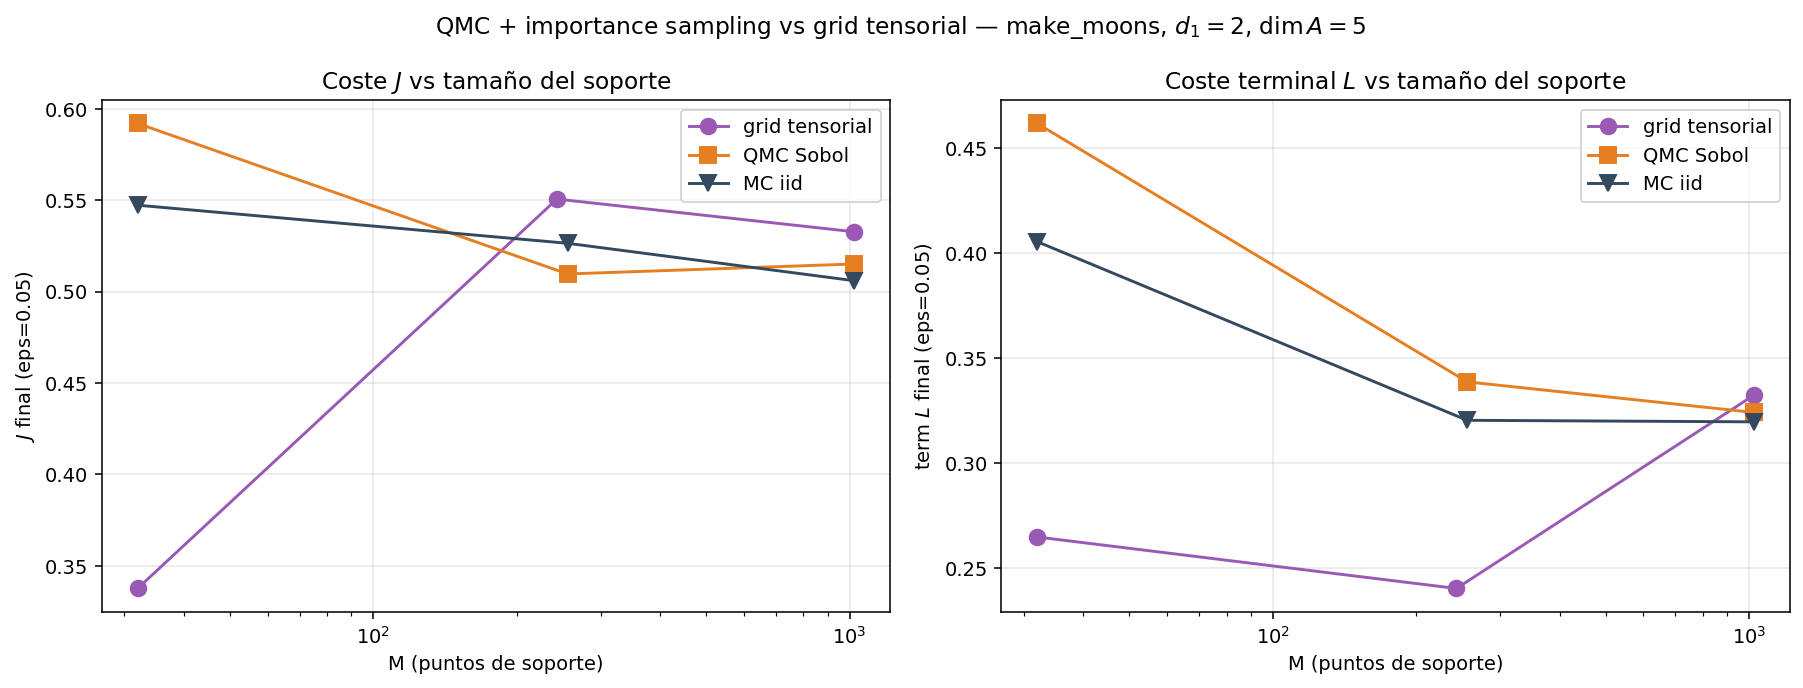
\includegraphics[width=0.95\textwidth]{../figures/04_qmc_convergence.png}
\caption{Coste $J$ y término terminal $L$ vs tamaño del soporte
$M$ (escala log). Para $M\geq 256$ las tres familias convergen
al mismo valor; QMC y MC son indistinguibles en este régimen,
pero ambos baten al grid tensorial en eficiencia
\emph{tiempo/calidad}.\label{fig:qmc-convergence}}
\end{figure}

Lectura: en $d_1=2$ el grid sigue siendo viable y la ganancia
es modesta ($\sim 4\times$ tiempo). El interés real está en
$d_1\geq 3$, donde la cuadratura tensorial empieza a no caber
en memoria pero $N$ puede mantenerse fijo en
QMC/MC --- esto vuelve viables comparaciones cuantitativas en
$d_1\in\{3,4,5\}$ que el grid no permite.

\paragraph{Otras alternativas (no implementadas).}
Dos familias adicionales podrían subir más el techo dimensional:

\begin{itemize}
  \item \textbf{Sparse grids (Smolyak)}. Escalan
        $\mathcal O(N\,(\log N)^{d-1})$ en lugar de
        $\mathcal O(N^d)$. Cada iteración Picard cambia
        $\varphi$, por lo que conviene combinar Smolyak con
        refinamiento dimensional adaptativo
        (\emph{combination technique}). Esfuerzo medio,
        librerías estándar (Tasmanian, sparseSpACE).
  \item \textbf{Tensor trains (TT-cross)}. La estructura
        $b(x,a)=\tanh(a_1\!\cdot\!x + a_2)\cdot a_0$ separa
        $a_0$ (entra linealmente) de $(a_1,a_2)$ (entran por
        $\tanh$), lo que \emph{sugiere} rango TT bajo. Si se
        confirma, el coste pasa a
        $\mathcal O(d\cdot r^2 \cdot n)$ y
        $d_1=8$ se vuelve viable. El coste de
        $\varphi(a)=\E_\gamma[b\cdot\nabla_x u]$ introduce
        acoplamiento adicional que podría degradar el rango;
        el riesgo es alto, el \emph{payoff} potencialmente
        transformador.
\end{itemize}

Ninguna de estas alternativas vuelve competitivo al solver
explícito frente al método paramétrico de la
Sección~\ref{sec:reg-moons}: cada iteración Picard reconstruye
el integrando, mientras que el optimizador paramétrico aprovecha
vectorización GPU sobre mini-batches. El interés conceptual
\---comparar $\nu^*_t$ exacta vs.\ histogramas empíricos en
dimensiones moderadas\--- es el que motiva todo el bloque, y se
materializa parcialmente en la Sección~\ref{sec:bridge}.

% ============================================================
\section{Regularizadores sobre \texttt{make\_moons}: SGLD,
pSGLD, MMD$^2$ y Sinkhorn}
\label{sec:reg-moons}

En la Sección~\ref{sec:explicita} se aplicó la fórmula explícita
del Teorema~1.4 a problemas $1\!\to\!1$ donde el coste terminal
$L(x,y)=\tfrac12(x-y)^2$ y la dimensión del estado coinciden con
las del paper. En esta sección se aborda
\texttt{make\_moons} ($d_1=2$, etiquetas binarias) por dos vías
complementarias:
\begin{enumerate}
  \item[(A)] Aproximaciones \emph{paramétricas} basadas en
        \texttt{MeanFieldResNet}, donde la medida $\nu_t$ se
        sustituye por $M$ partículas $(\theta^m)$. La penalización
        $\eps\,\mathcal E(\nu_t\|\nu^\infty)$ es estrictamente
        infinita en este régimen (Sección~\ref{sec:reg-moons-kl}),
        de manera que se exploran cuatro \emph{sustitutos} bien
        definidos: SGLD vanilla, pSGLD, MMD$^2$ y Sinkhorn.
  \item[(B)] Resolución \emph{explícita} (extensión $n$-D del
        algoritmo de la Sección~\ref{sec:explicita}) sobre
        \texttt{make\_moons} con un \emph{embedding} de etiquetas
        $y\in\{0,1\}\mapsto y_{\text{emb}}\in\mathbb{R}^2$, lo que
        encaja exactamente en el Ejemplo~1.3 del paper
        ($d_1=d_2=2$).
\end{enumerate}

\subsection{Obstrucción KL$=+\infty$ y motivación}
\label{sec:reg-moons-kl}

La penalización entrópica del paper es
\[
  \mathcal E(\nu_t\|\nu^\infty) \;=\; \int \log\frac{d\nu_t}{d\nu^\infty}\,d\nu_t,
  \qquad \nu^\infty(da)\propto e^{-\ell(a)}\,da.
\]
En la implementación con $M$ partículas $\nu_t = \tfrac1M\sum_m\delta_{\theta^m(t)}$
se tiene $\nu_t \perp \nu^\infty$ (la primera es discreta y la
segunda absolutamente continua), de modo que
$\mathrm{KL}(\nu_t\|\nu^\infty)=+\infty$ y $\mathcal E$ no se puede
evaluar literalmente. Se contemplan tres familias de sustitutos:
\begin{itemize}
  \item \textbf{Energía supercoerciva} (sin término entrópico):
        $\mathcal E_{\text{aprox}}(\nu_t)=
        \tfrac1{N_p}\sum_j \ell(\theta_j)$.
        Equivale a regularización $L^2+L^4$ sobre los pesos.
        \emph{Pierde} el componente $-\mathcal H(\nu_t)$ de la
        entropía diferencial.
  \item \textbf{Ruido de Langevin} (SGLD/pSGLD): se inyecta
        $\sqrt{2\eta\eps M_t}\,\xi$ tras cada paso del optimizador.
        La cadena $(\theta_t)$, con $\theta\in\mathbb{R}^{M(2d_1+1)}$
        (los $M$ pesos concatenados), tiene como medida estacionaria
        $\nu^*_{\mathrm{SGLD}}(\theta)\propto \exp(-J(\theta)/\eps)$.
        \emph{No} es literalmente la $\nu^*_t$ del Teorema 1.4 (que
        vive en $\mathcal A=\mathbb{R}^{2d_1+1}$ y depende de $t$),
        sino su \emph{análogo finito-dimensional} en la
        parametrización $M$-partículas: cuando $M\to\infty$, la
        medida empírica $\tfrac1M\sum\delta_{a_i}$ de un sample
        $\theta\sim\nu^*_{\mathrm{SGLD}}$ tiende, formalmente, al
        objeto continuo del paper (propagación de caos).
  \item \textbf{Distancias entre medidas} (MMD$^2$, Sinkhorn): se
        sustituye $\mathcal E(\nu_t\|\nu^\infty)$ por una distancia
        bien definida entre $\nu_t$ (partículas) y muestras del
        prior $\nu^\infty$ obtenidas por ULA.\footnote{ULA
        (\emph{Unadjusted Langevin Algorithm}) es la discretización
        Euler-Maruyama de la SDE de Langevin
        $d\theta_t = -\nabla U(\theta_t)\,dt + \sqrt{2}\,dW_t$:
        $\theta_{k+1} = \theta_k - \eta\,\nabla U(\theta_k)
        + \sqrt{2\eta}\,\xi_k$ con $\xi_k\sim\mathcal N(0,I)$.
        Su distribución estacionaria aproxima
        $\propto\exp(-U(\theta))$; el calificativo ``unadjusted''
        se debe a que ---a diferencia de MALA--- omite el paso
        Metropolis-Hastings que corrige el sesgo de discretización,
        a cambio de mayor velocidad y simplicidad
        \cite{RobertsTweedie1996,Durmus2017}. Aquí lo usamos con
        $U=\ell/\eps$ para obtener un \emph{sample} cuasi-i.i.d.\ de
        $\nu^\infty$ que sirva de referencia para los regularizadores
        MMD$^2$ y Sinkhorn.}
\end{itemize}

\subsection{SGLD vanilla y por qué no basta}
\label{sec:reg-moons-sgld}

La actualización SGLD de libro de texto es
\[
  \theta_{t+1} \;=\; \theta_t - \eta\,\nabla J(\theta_t) +
  \sqrt{2\eta\eps}\,\xi_t,\qquad \xi_t\sim\mathcal{N}(0,I).
\]
Su distribución estacionaria es
$\nu^*_{\mathrm{SGLD}}(\theta)\propto\exp(-J(\theta)/\eps)$ sobre
$\theta\in\mathbb{R}^{M(2d_1+1)}$ (no la $\nu^*_t$ del paper; cf.\
discusión arriba). En la \texttt{MeanFieldResNet} sobre
\texttt{make\_moons} esto falla en la práctica:
\begin{itemize}
  \item Los gradientes de la BCE están en escala $\sim 10^{-5}$
        mientras que el ruido $\sqrt{2\eta\eps}\sim 10^{-3}$ los
        domina en cada paso.
  \item Sin precondicionamiento, las direcciones planas y empinadas
        reciben el mismo paso $\eta$, lo que estanca a
        $\theta_t$ en regiones de alta pérdida.
\end{itemize}
Esto se confirma empíricamente: tras 800 épocas con $\eps=0.01$ y
$\eta=10^{-3}$, SGLD vanilla queda en $J\approx 0.48$ y precisión
$\approx 0.87$, frente a $J\lesssim 0.01$ y precisión $1.000$ que
alcanzan los demás métodos (Tabla~\ref{tab:reg-moons}).

\subsection{pSGLD (Li et al.\ 2016)}
\label{sec:reg-moons-psgld}

Sea $v_t$ el segundo momento sesgo-corregido de Adam, y
$M_t = \min\!\bigl(1/(\sqrt{\hat v_t}+\delta),\,1\bigr)$ el
precondicionador (\emph{clamp} a 1 para evitar explosión del ruido en
direcciones planas). pSGLD es
\[
  \theta_{t+1} \;=\; \mathrm{Adam}(\theta_t,\nabla J(\theta_t)) +
  \sqrt{2\eta\eps\,M_t}\,\xi_t.
\]
El acoplamiento $\sqrt{M_t}$ es esencial: el ruido isótropo
desacoplaría la cadena del precondicionador y destruiría la medida
estacionaria. Con $M_t\le 1$, pSGLD aproxima el muestreo de
$\nu^*_{\mathrm{SGLD}}\propto\exp(-J/\eps)$ bajo la métrica inducida
por $M_t$, lo que en la práctica equivale a inyectar la cantidad
correcta de exploración entrópica sin destruir la convergencia del
optimizador.

\begin{remark}[pSGLD es un sampler aproximado]
\label{rem:psgld-aprox}
Estrictamente, una cadena de Langevin precondicionada por una matriz
$G(\theta)$ \emph{espacialmente variable} sólo preserva la medida
$\propto\exp(-J/\eps)$ si la deriva incluye el término correctivo
$\eps\,\nabla\!\cdot G(\theta)$ \cite{Ma2015,Girolami2011}. La
formulación práctica de pSGLD~\cite{Li2016} omite o aproxima ese
término, por lo que su distribución estacionaria está \emph{cerca}
de $\exp(-J/\eps)$ pero no coincide exactamente. Esta es la razón por
la que en todo el texto nos referimos a pSGLD como heurística
``\emph{alineada}'' con el muestreo Gibbs en lugar de
``\emph{realización rigurosa}'' del mismo.
\end{remark}

\subsection{Regularizador MMD$^2$}
\label{sec:reg-moons-mmd}

\paragraph{Definición.} La \emph{Maximum Mean Discrepancy} al
cuadrado entre dos distribuciones $P, Q$ sobre $\R^d$, asociada a un
kernel positivo definido $K$ con RKHS $\mathcal H_K$, es
\cite{Gretton2012}
\[
  \mathrm{MMD}^2(P, Q) \;:=\;
  \bigl\| \mu_P - \mu_Q \bigr\|_{\mathcal H_K}^2
  \;=\;
  \E_{x,x'\sim P}[K(x,x')] - 2\,\E_{x\sim P, y\sim Q}[K(x,y)]
  + \E_{y,y'\sim Q}[K(y,y')],
\]
donde $\mu_P = \E_{x\sim P}[K(x,\cdot)] \in \mathcal H_K$ es el
\emph{mean embedding} de $P$. Para kernels característicos (e.g.,
Gaussiano), $\mathrm{MMD}^2(P,Q)=0 \iff P=Q$, por lo que es una
métrica genuina entre distribuciones. A diferencia de la KL, está
bien definida entre medidas singulares y absolutamente continuas
---en particular entre la empírica $\nu^{(M)}$ y el prior continuo
$\nu^\infty$--- que es justo lo que necesitamos.

\paragraph{Estimador empírico.} Dadas $X = (x_m)_{m=1}^M$ partículas
(neuronas $\theta^m$) y $Y = (y_n)_{n=1}^N$ muestras i.i.d.\ de
$\nu^\infty$ (obtenidas por ULA con potencial $U=\ell/\eps$),
sustituimos las esperanzas por promedios sobre las muestras. El
estimador \emph{V-statistic} (sesgado, incluye los términos
diagonales $i=j$) es
\[
  \widehat{\mathrm{MMD}}^2_\sigma(X, Y) \;=\;
  \tfrac{1}{M^2}\!\sum_{i,j=1}^M\! K_\sigma(x_i, x_j)
  - \tfrac{2}{M N}\!\sum_{i=1}^M\!\sum_{j=1}^N\! K_\sigma(x_i, y_j)
  + \tfrac{1}{N^2}\!\sum_{i,j=1}^N\! K_\sigma(y_i, y_j),
\]
con kernel Gaussiano
$K_\sigma(x, y) = \exp\!\bigl(-\|x - y\|^2/(2\sigma^2)\bigr)$.
Usamos la versión sesgada (V-statistic) en vez de la insesgada
(U-statistic, que excluye $i=j$) porque (a) tiene varianza menor,
(b) es siempre $\geq 0$ y por tanto un objetivo de optimización bien
condicionado, y (c) el sesgo $\mathcal O(1/M)$ es despreciable frente
al efecto del término BCE en el coste total
\cite{Gretton2012,Sutherland2017}. Coste: $\mathcal O((M+N)^2 d)$ por
mini-batch.

\paragraph{Elección del bandwidth $\sigma$.} Aplicamos la
\emph{heurística de la mediana}~\cite{Gretton2012}:
$\sigma^2 = \tfrac{1}{2}\,\mathrm{median}\bigl\{\|z_i - z_j\|^2 :
z_i, z_j \in X \cup Y,\ i\neq j\bigr\}$, calculada \emph{una sola vez}
al inicio del entrenamiento sobre un sample inicial $X^{(0)}$. Fijar
$\sigma$ es importante: si se actualizase con $X$ a lo largo del
entrenamiento, el paisaje de pérdida dejaría de ser estacionario y
los gradientes serían inconsistentes. La heurística da un
$\sigma$ del orden de la dispersión típica entre puntos del soporte
combinado, lo que evita los dos regímenes degenerados:
$\sigma\to 0$ (kernel se vuelve $\delta$, MMD$^2$ no detecta
similitud) y $\sigma\to\infty$ (kernel constante, MMD$^2$ no
distingue distribuciones).

\paragraph{Coste de entrenamiento.} El coste minimizado es
\[
  J_{\mathrm{MMD}}(\theta) \;=\;
  \underbrace{\mathcal L_{\mathrm{BCE}}(\theta)}_{\text{predictivo}}
  \;+\; \eps\cdot \widehat{\mathrm{MMD}}^2_\sigma(X(\theta), Y),
\]
donde $X(\theta)$ son las neuronas efectivas (a $t=T$ tras la
augmentación temporal) inducidas por $\theta$. El término
$\sum_{i,j}\! K_\sigma(y_i, y_j)$ no depende de $\theta$ y se
precomputa al inicio. Solo los dos primeros términos del estimador
contribuyen al gradiente.

\subsection{Divergencia de Sinkhorn debiased}
\label{sec:reg-moons-sinkhorn}

\paragraph{Transporte óptimo entrópico.} Dado un coste
$c: \R^d\times\R^d\to\R_{\geq 0}$ (aquí $c(x,y)=\|x-y\|^2$,
normalizado a $[0,1]$ por estabilidad), el problema de Kantorovich
clásico es
\[
  \mathrm{OT}(\mu,\nu) \;=\; \min_{\pi\in\Pi(\mu,\nu)}
  \int c(x,y)\,d\pi(x,y),
\]
donde $\Pi(\mu,\nu)$ son las medidas de probabilidad sobre
$\R^d\times\R^d$ con marginales $\mu$ y $\nu$.
Cuturi~\cite{Cuturi2013} introdujo la regularización entrópica con
parámetro $\eps_{\mathrm{ot}}>0$ (el \texttt{blur} en
\texttt{geomloss}):
\[
  \mathrm{OT}_{\eps_{\mathrm{ot}}}(\mu,\nu)
  \;=\; \min_{\pi\in\Pi(\mu,\nu)}
  \int c(x,y)\,d\pi(x,y)
  \;+\; \eps_{\mathrm{ot}}\cdot \mathrm{KL}(\pi\,\|\,\mu\otimes\nu).
\]
La inclusión del término entrópico convierte el LP original en un
problema estrictamente convexo y diferenciable, resoluble por
iteraciones de \emph{Sinkhorn-Knopp} en el dominio dual (escalado
matricial alternado), con coste $\mathcal O(N^2)$ por iteración y
~$\mathcal O(\log(1/\delta))$ iteraciones en el régimen estable.

\begin{remark}[¿Por qué usar Sinkhorn si lleva una KL dentro?]
\label{rem:sinkhorn-kl}
A primera vista parece circular: queremos evitar
$\mathrm{KL}(\nu_t \| \nu^\infty) = +\infty$ (Sección~\ref{sec:reg-moons-kl})
y para ello introducimos un funcional que \emph{también} contiene
una KL. La diferencia es esencial:
\begin{itemize}
  \item La KL problemática es
        $\mathrm{KL}(\nu^{(M)} \,\|\, \nu^\infty)$ entre la
        \emph{empírica de partículas} (singular, soporte de
        medida nula) y el \emph{prior continuo}. Es $+\infty$
        porque $\nu^{(M)}$ no es absolutamente continua respecto
        de $\nu^\infty$.
  \item La KL dentro de Sinkhorn es
        $\mathrm{KL}(\pi \,\|\, \mu\otimes\nu)$ entre el
        \emph{plan de transporte} $\pi$ y la \emph{medida producto}
        de las marginales, no entre $\mu$ y $\nu$ directamente.
        Cuando $\mu = \tfrac1M\sum\delta_{x_m}$ y
        $\nu = \tfrac1N\sum\delta_{y_n}$ son discretas, todo
        $\pi\in\Pi(\mu,\nu)$ vive en el soporte finito
        $\{x_m\}\times\{y_n\}$, y por construcción
        $\pi\ll\mu\otimes\nu$. Entonces
        $\mathrm{KL}(\pi\|\mu\otimes\nu)<+\infty$
        \emph{automáticamente}, sin importar la estructura de
        $\mu, \nu$.
\end{itemize}
Es decir, Sinkhorn redirige la regularización entrópica al espacio
de \emph{couplings} (donde la KL siempre es finita) en vez de
aplicarla al espacio de \emph{distribuciones marginales} (donde la
KL contra $\nu^\infty$ explota). Esa es la jugada conceptual que lo
hace viable como proxy del término entrópico de Daudin-Delarue.
\end{remark}

\paragraph{Sinkhorn debiased.} El funcional
$\mathrm{OT}_{\eps_{\mathrm{ot}}}$ tiene un sesgo entrópico molesto:
$\mathrm{OT}_{\eps_{\mathrm{ot}}}(\mu,\mu) \neq 0$ en general, y de
hecho favorece distribuciones \emph{difusas} (entropy-blurred). La
divergencia de Sinkhorn \emph{debiased} de
Genevay--Peyré--Cuturi~\cite{Genevay2018,Feydy2019} corrige esto
sustrayendo los términos diagonales:
\[
  S_{\eps_{\mathrm{ot}}}(\mu,\nu) \;=\;
  \mathrm{OT}_{\eps_{\mathrm{ot}}}(\mu,\nu)
  \;-\; \tfrac12\,\mathrm{OT}_{\eps_{\mathrm{ot}}}(\mu,\mu)
  \;-\; \tfrac12\,\mathrm{OT}_{\eps_{\mathrm{ot}}}(\nu,\nu).
\]
Esta versión satisface (i) $S_{\eps_{\mathrm{ot}}}(\mu,\nu)\geq 0$,
(ii) $S_{\eps_{\mathrm{ot}}}(\mu,\nu)=0\iff \mu=\nu$, y (iii)
interpola entre $\mathrm{OT}$ ($\eps_{\mathrm{ot}}\to 0$, transporte
óptimo) y MMD$^2$ con el kernel $-\|x-y\|^2$
($\eps_{\mathrm{ot}}\to\infty$)~\cite{Feydy2019}. En este sentido
es una familia de divergencias \emph{geométricas} indexadas por la
intensidad de regularización.

\paragraph{Implementación.} Usamos la versión \emph{log}-Sinkhorn
(estabilidad en log-sumexp) con coste cuadrático normalizado a
$[0,1]$, $50$ iteraciones internas, y $\texttt{blur}=
\eps_{\mathrm{ot}}=0.05$. El término diagonal
$\mathrm{OT}_{\eps_{\mathrm{ot}}}(Y, Y)$ no depende de $\theta$ y se
precomputa una vez sobre el sample de $\nu^\infty$ (obtenido por
ULA, igual que en MMD$^2$). El coste de entrenamiento es análogo:
\[
  J_{\mathrm{Sink}}(\theta) \;=\;
  \mathcal L_{\mathrm{BCE}}(\theta)
  \;+\; \eps\cdot S_{\eps_{\mathrm{ot}}}\bigl(X(\theta),\,Y\bigr).
\]
Frente a MMD$^2$, Sinkhorn capta mejor la \emph{geometría} del
soporte en $\R^5$ ---compara distribuciones penalizando el coste de
\emph{mover} masa, no solo la distancia entre \emph{mean
embeddings}--- a costa de mayor latencia por iteración (las $50$
iteraciones internas frente al estimador en forma cerrada de MMD$^2$).

\subsection{Comparación experimental}
\label{sec:reg-moons-exp}

\textbf{Setup.} \texttt{make\_moons} con $N=400$,
\texttt{noise}$=0.12$, $M=64$ partículas, $K=10$ pasos
RK4, $T=1$, $\eps=0.01$, $800$ épocas, semilla
\texttt{torch.manual\_seed(42)}. Las muestras del prior
$Y\in\mathbb R^5$ ($n=400$) se obtienen por ULA fuera del bucle de
entrenamiento. Los cuatro métodos comparten la misma red y la misma
semilla; la única diferencia es el regularizador.

\begin{table}[H]
\centering
\begin{tabular}{lrrr}
\toprule
método & $J^\star$ & accuracy final & $J$ finito \\
\midrule
SGLD vanilla       & $0.481$ & $0.868$ & sí \\
pSGLD              & $0.0017$ & $1.000$ & sí \\
MMD$^2$            & $0.0029$ & $1.000$ & sí \\
Sinkhorn debiased  & $0.0063$ & $1.000$ & sí \\
\bottomrule
\end{tabular}
\caption{Comparación de regularizadores sobre \texttt{make\_moons}
con la \texttt{MeanFieldResNet} ($\eps=0.01$, $800$ épocas, misma
semilla). SGLD vanilla queda atrapado; pSGLD/MMD/Sinkhorn convergen
a precisión perfecta. \label{tab:reg-moons}}
\end{table}

\begin{figure}[H]
\centering
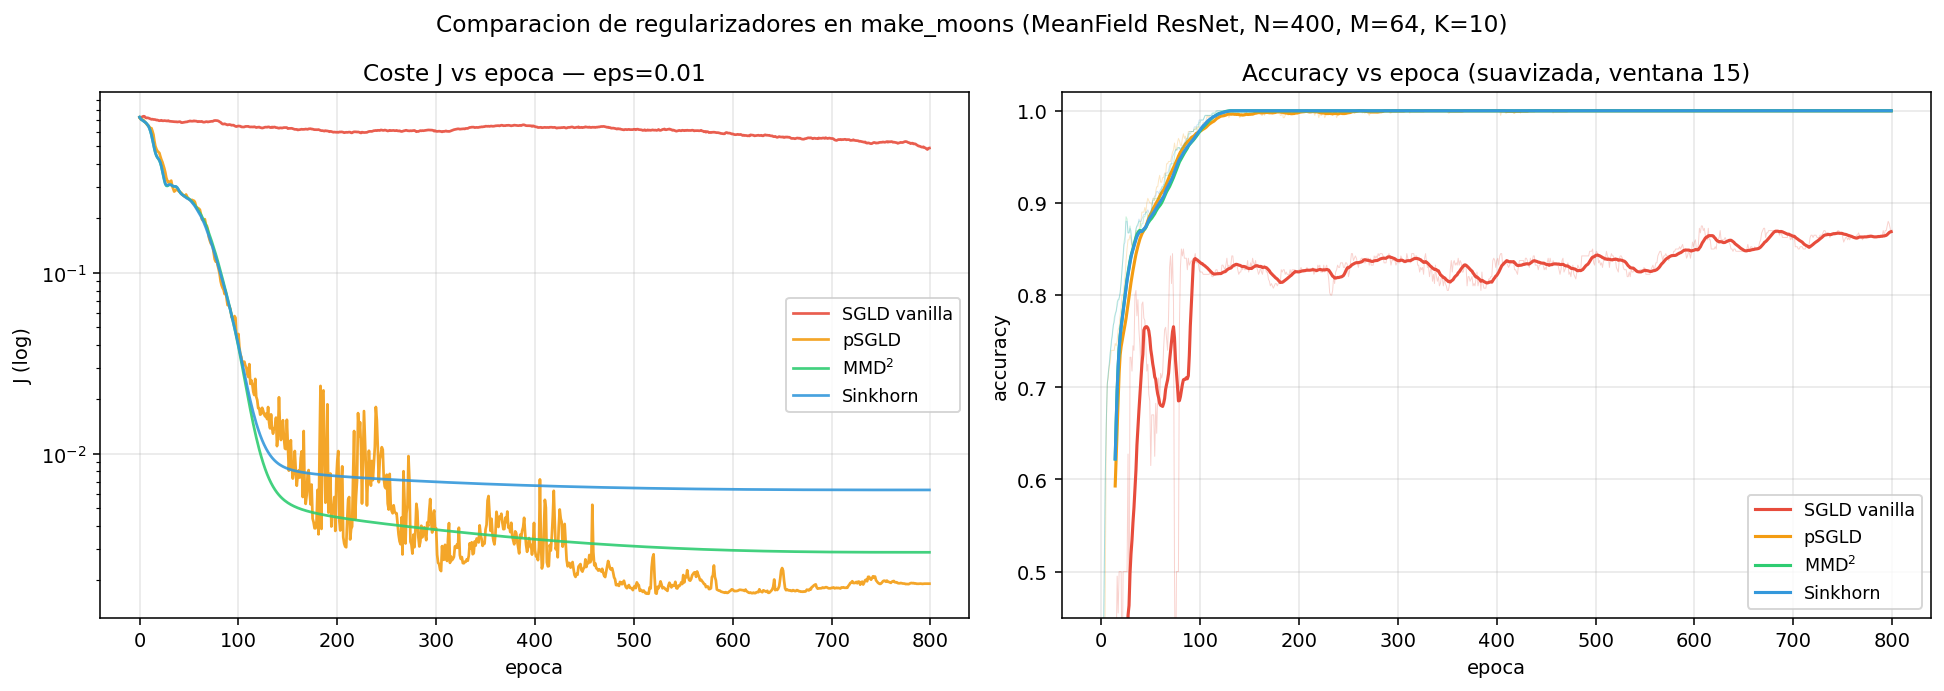
\includegraphics[width=0.95\textwidth]{../figures/02_metodos_comparacion.png}
\caption{Curvas $J(t)$ (escala log) y \emph{accuracy} suavizada
(ventana 15) por método sobre \texttt{make\_moons}. SGLD vanilla
queda en una meseta de pérdida alta; los tres regularizadores
restantes alcanzan $J<0.01$ en menos de 200 épocas.
\label{fig:reg-moons-curvas}}
\end{figure}

\begin{figure}[H]
\centering
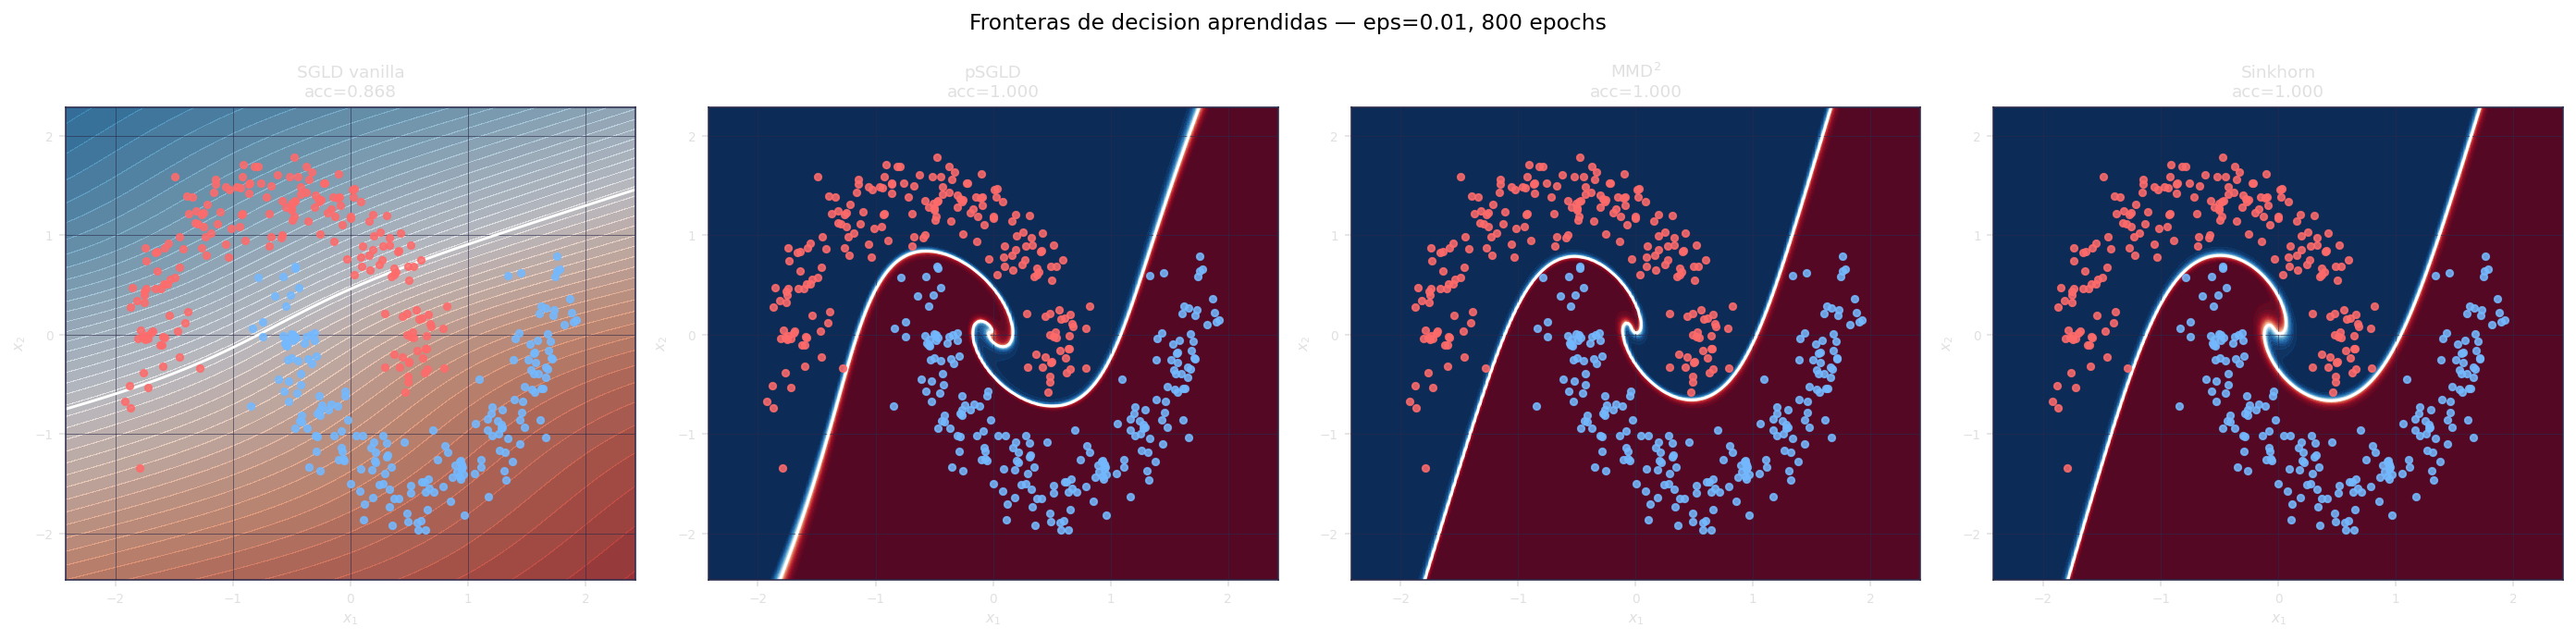
\includegraphics[width=0.95\textwidth]{../figures/02_metodos_fronteras.png}
\caption{Fronteras de decisión aprendidas por los cuatro métodos.
SGLD vanilla deja regiones grandes mal clasificadas; los demás
producen fronteras curvas que separan completamente las dos
medias lunas.\label{fig:reg-moons-fronteras}}
\end{figure}

\subsection{Solución explícita en \texttt{make\_moons}: extensión $n$-D}
\label{sec:reg-moons-explicit}

\paragraph{Embedding de etiquetas.}
Para encajar \texttt{make\_moons} en el setup del paper
($d_1=d_2$, coste $L(x,y)=\tfrac12|x-y|^2$) se embebe
$y\in\{0,1\}$ en $\mathbb R^2$:
\[
  y \;\longmapsto\; y_{\mathrm{emb}} =
  \begin{cases}
    (-1, 0) & \text{si } y=0,\\
    (\,+1, 0) & \text{si } y=1.
  \end{cases}
\]
Así $X(T)\in\mathbb R^2$ debe acercarse al \emph{ancla} de su clase,
y la regla de clasificación es $\widehat y = \mathbf 1\{X_1(T) > 0\}$.

\paragraph{Generalización del solver a $d_1\ge 1$.}
La fórmula del Teorema~1.4 se mantiene literalmente; cambian las
dimensiones de los objetos:
\begin{align*}
  b(x,a) &= \tanh(a_1\!\cdot\! x + a_2)\,a_0
  \;\in\;\mathbb R^{d_1},\quad a=(a_0,a_1,a_2)\in\mathbb R^{2d_1+1},\\
  \tfrac{\partial b_k}{\partial x_j}(x,a) &=
  \mathrm{sech}^2(a_1\!\cdot\! x + a_2)\,a_{1,j}\,a_{0,k},\\
  \tfrac{d}{dt} \Phi_i(t) &= (\partial_x \bar b)\bigl(X_i(t),\nu_t\bigr)\,\Phi_i(t),
  \qquad \Phi_i(0) = I_{d_1}.
\end{align*}
El gradiente de la función valor por características usa el cocycle
de la matriz Jacobiana del flujo:
\[
  \nabla_x u_t^*\bigl(X_i(t), y_i\bigr) =
  \bigl(\Phi_i(T)\,\Phi_i(t)^{-1}\bigr)^{\!\top}\,(X_i(T) - y_i),
\]
que generaliza la fórmula escalar de la Sección~\ref{sec:explicita}.
La fórmula de Gibbs es idéntica:
\[
  \nu_t^*(a) \;\propto\;
  \exp\!\Bigl(-\ell(a) -
    \tfrac1\eps\,\tfrac1N\sum_{i=1}^N
    b\bigl(X_i(t),a\bigr)\!\cdot\!\nabla_x u_t^*(X_i(t),y_i)\Bigr).
\]

\paragraph{Discretización del grid.}
Con $d_1=2$, el espacio de parámetros es $A=\mathbb R^5$. Un
\emph{grid} uniforme con $M_{\mathrm{pd}}$ puntos por dimensión da
$M=M_{\mathrm{pd}}^5$ puntos totales. Por requisitos de memoria y
tiempo se usa $M_{\mathrm{pd}}=4$ y $R=2$, es decir, $M=1\,024$
puntos en $[-2,2]^5$. El \emph{warm-start} de la continuación en
$\eps$ y RK4 con $K=10$ pasos completan la discretización.

\paragraph{Resultados.}
La Tabla~\ref{tab:explicit-moons} resume la continuación en
$\eps$ con $M_{\mathrm{pd}}=4$ ($M=1\,024$). El tiempo total de
las cinco corridas es $\sim 4.6$ minutos en CPU.

\begin{table}[H]
\centering
\begin{tabular}{lrrrrr}
\toprule
$\eps$ & iters & conv & $J$ & term $L$ & acc \\
\midrule
$0.50$ & $26$  & sí & $0.842$ & $0.753$ & $0.69$ \\
$0.20$ & $26$  & sí & $0.752$ & $0.612$ & $0.71$ \\
$0.10$ & $27$  & sí & $0.654$ & $0.472$ & $0.75$ \\
$0.05$ & $38$  & sí & $0.533$ & $0.332$ & $0.81$ \\
$0.02$ & $150$ & no & $0.383$ & $0.193$ & $0.89$ \\
\bottomrule
\end{tabular}
\caption{Solución explícita en \texttt{make\_moons} por
continuación en $\eps$. La precisión \emph{acc} se mide como
$\mathbf 1\{X_1(T)>0\}=y$. Para $\eps=0.02$ la iteración Picard
alcanza el cap de $150$ iteraciones sin estabilizarse en TV (igual
patrón que en la Sección~\ref{sec:explicita}: $\eps$ pequeños
exigen un grid más fino o un esquema de continuación más conservador),
pero la accuracy ya es $0.89$.\label{tab:explicit-moons}}
\end{table}

\begin{figure}[H]
\centering
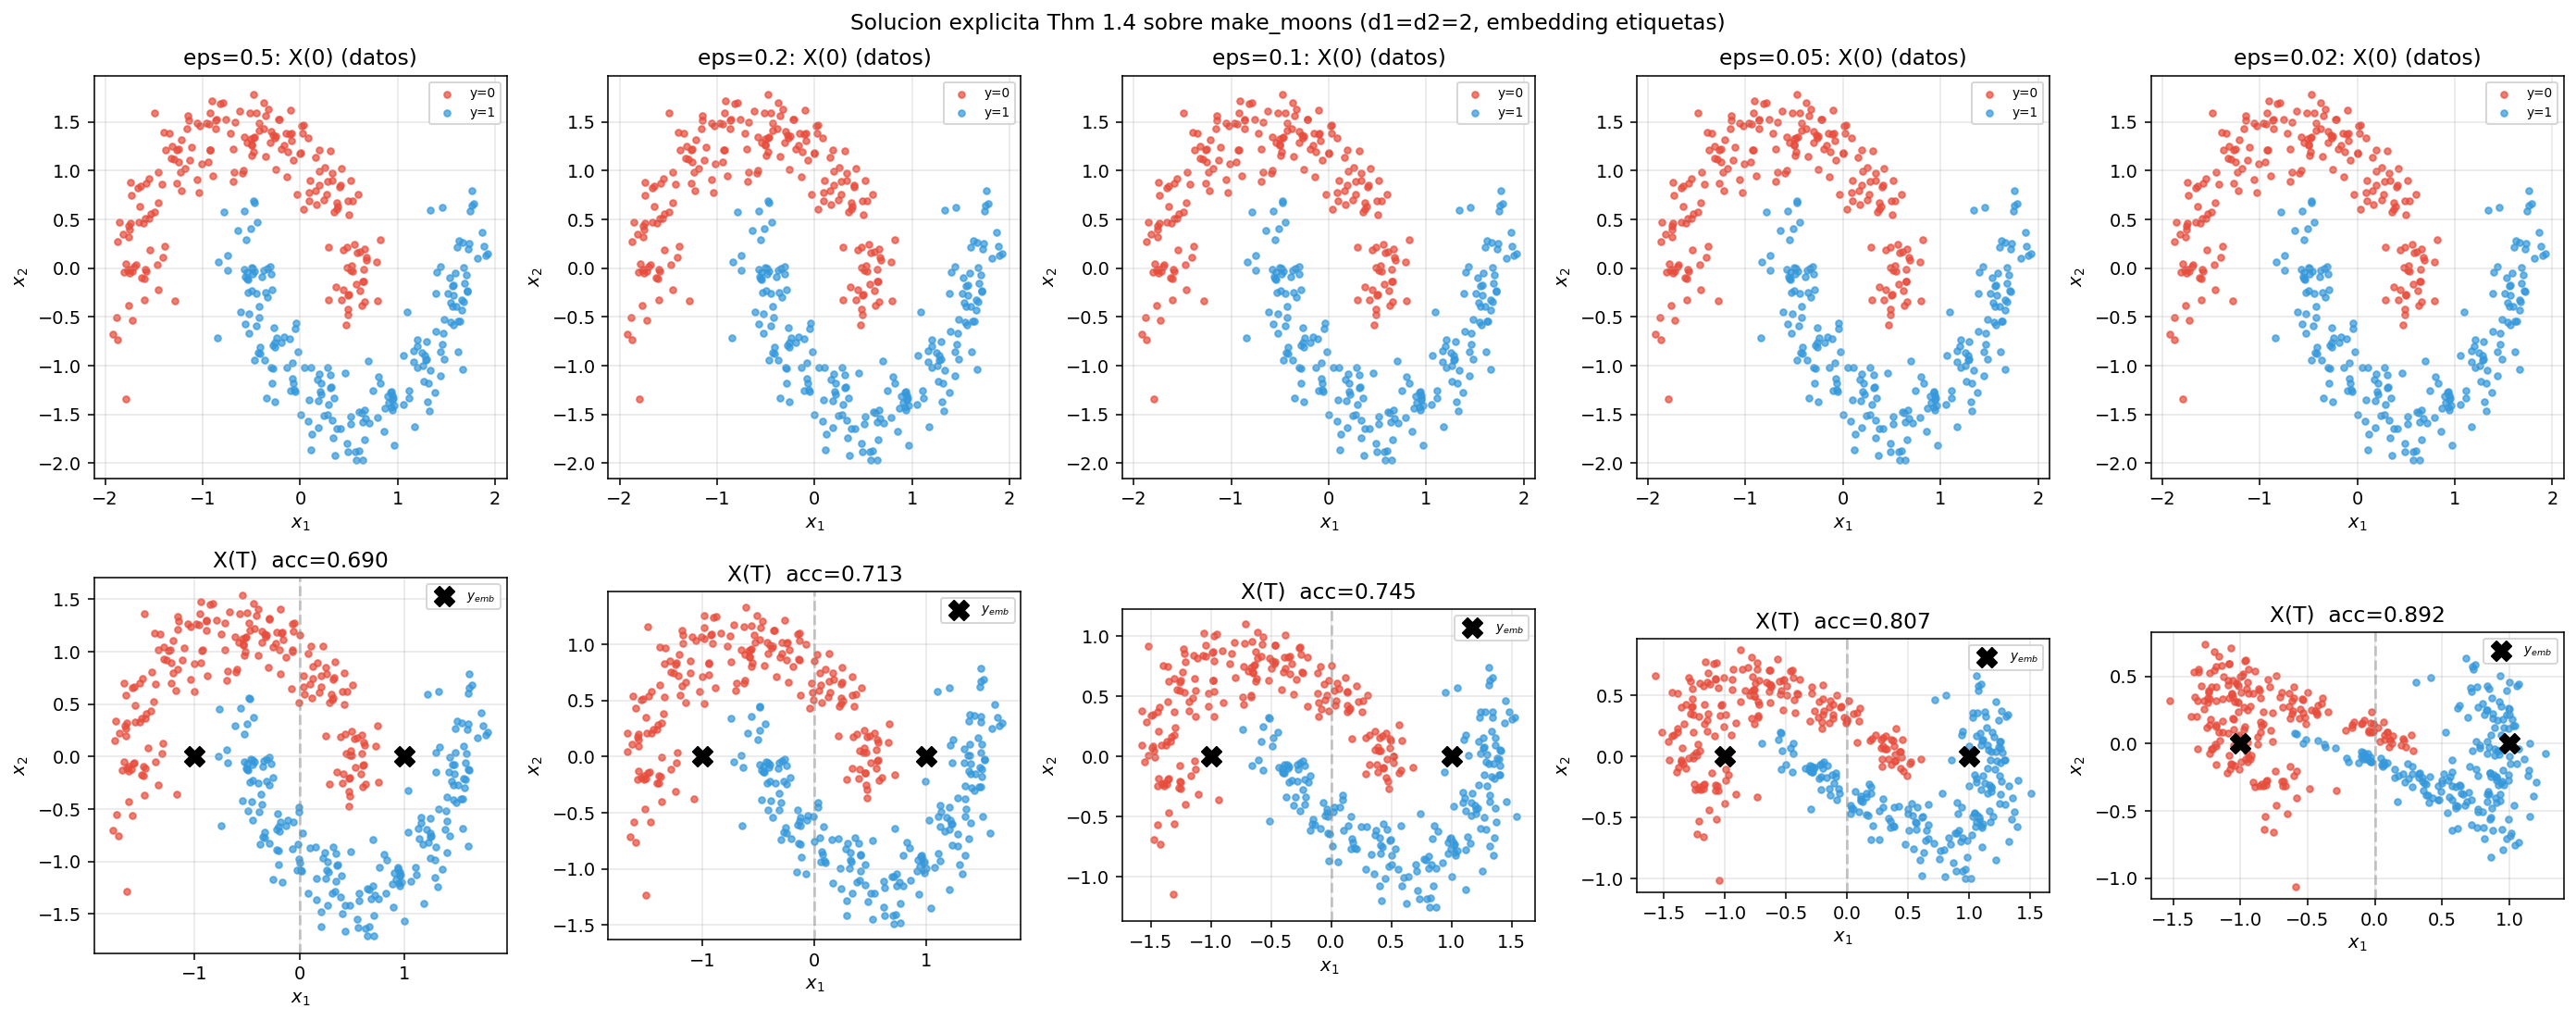
\includegraphics[width=0.95\textwidth]{../figures/02_explicit_moons.png}
\caption{Fila superior: $X(0)$ (datos originales \texttt{make\_moons})
para cada $\eps$ de la continuación; fila inferior: $X(T)$ (predicción
del flujo) coloreado por clase, con anclas $y_{\mathrm{emb}}=(\pm 1,0)$
en negro. A medida que $\eps$ disminuye, la población se separa hacia
sus respectivas anclas y la línea $X_1(T)=0$ funciona como frontera
de clasificación.\label{fig:explicit-moons}}
\end{figure}

\begin{figure}[H]
\centering
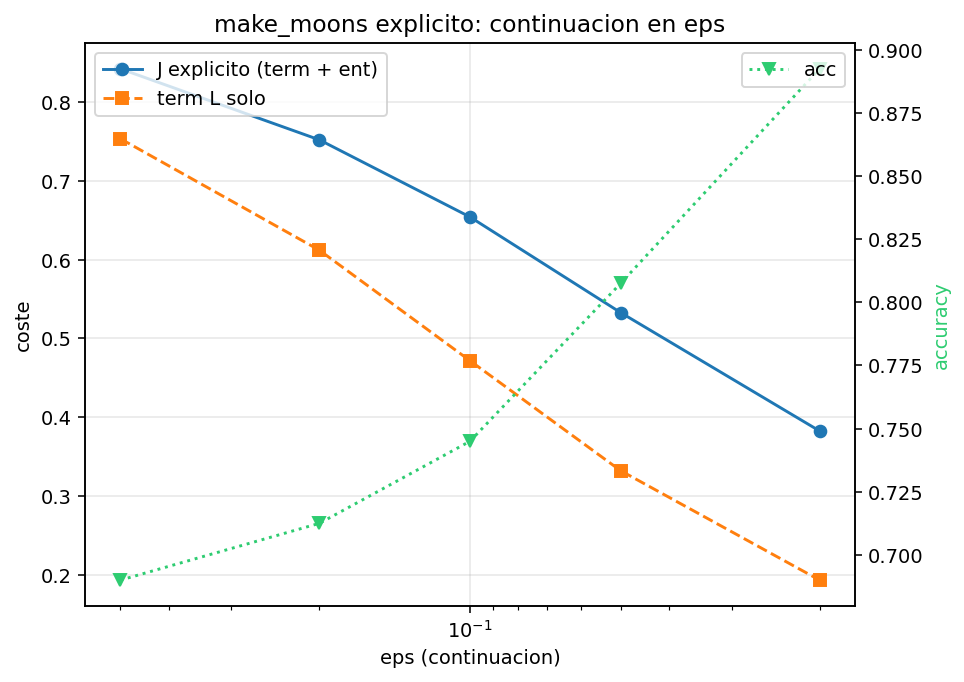
\includegraphics[width=0.65\textwidth]{../figures/02_explicit_moons_curves.png}
\caption{Coste $J(\eps)$ y término terminal $L$ (escala log invertida
en $\eps$) junto con la accuracy. Ambos costes decrecen
monótonamente al reducir $\eps$ y la accuracy crece hasta $0.89$.
Comparado con \texttt{MeanFieldResNet} (Tabla~\ref{tab:reg-moons}),
el solver explícito alcanza menor accuracy porque el grid finito
$M=1\,024$ en $[-2,2]^5$ no puede igualar los $M=64$ parámetros
\emph{libres} de la red.\label{fig:explicit-moons-curves}}
\end{figure}

\paragraph{Lectura comparativa.}
Las dos vías ofrecen información complementaria:
\begin{itemize}
  \item Las aproximaciones paramétricas
        (Sección~\ref{sec:reg-moons-exp}) son las que
        \emph{realmente convergen a $0$ pérdida} y por tanto las
        adecuadas para usar como predictor.
  \item El solver explícito (esta sección) es la \emph{única} vía que
        produce $\nu_t^*$ literal: en cada $t_k$ tenemos la
        distribución de Gibbs sobre el grid de $A$, lo que
        permite verificar empíricamente la fórmula del Teorema~1.4
        sin necesidad de muestreo Langevin ni de aproximaciones
        de la KL.
\end{itemize}

% ============================================================
\section{Regresión multivariada \emph{sin} PCA: California Housing en
$d_1=8$}
\label{sec:regresion-d8}

En el experimento G de la implementación A--K se aplicaba
\texttt{MeanFieldResNet} a California Housing tras una proyección
PCA(2): el modelo veía dos features sintéticas y la geometría
real (8 dimensiones) quedaba comprimida en el preprocesado. Esta
sección retira PCA y ejecuta los cuatro regularizadores
parámetricos sobre las 8 features originales estandarizadas, en
paralelo a tres baselines clásicos (OLS, Ridge, Random Forest).

\subsection{Setup}
\label{sec:reg-d8-setup}

\begin{itemize}
  \item Dataset: \texttt{fetch\_california\_housing} (8 features
        \texttt{MedInc}, \texttt{HouseAge}, \texttt{AveRooms},
        \texttt{AveBedrms}, \texttt{Population},
        \texttt{AveOccup}, \texttt{Latitude}, \texttt{Longitude}).
  \item $N_{\mathrm{train}}=800$, $N_{\mathrm{test}}=400$
        (subconjunto aleatorio fijado con \texttt{seed=42}).
  \item Estandarización separada de $X$ e $y$ (media $0$, std $1$).
  \item Modelo neural: \texttt{MeanFieldResNet} con $d_1=8$,
        $M=128$ partículas (frente a $M=64$ en \texttt{make\_moons}
        para compensar la mayor capacidad requerida en $d_1=8$),
        $K=10$ pasos RK4, $T=1$, $\eps=0.01$, $800$ épocas, misma
        \texttt{torch.manual\_seed(42)} en cada método.
  \item Prior $\nu^\infty$: $600$ muestras en $\mathbb R^{17}$
        ($\dim a = 2 d_1 + 1 = 17$) por ULA con $8\,000$ pasos de
        burn-in y \texttt{thin}$=20$.
  \item Baselines clásicos:
        \begin{itemize}
          \item \texttt{LinearRegression} (OLS, sklearn);
          \item \texttt{Ridge} con $\alpha=1.0$;
          \item \texttt{RandomForestRegressor} con $100$ árboles
                y \texttt{random\_state}$=42$.
        \end{itemize}
\end{itemize}

\subsection{Resultados}
\label{sec:reg-d8-resultados}

\begin{table}[H]
\centering
\begin{tabular}{lrrr}
\toprule
modelo & $R^2_{\text{train}}$ & $R^2_{\text{test}}$ & RMSE\textsubscript{test} \\
\midrule
OLS                 & $0.604$ & $0.626$ & $0.613$ \\
Ridge ($\alpha=1$)  & $0.604$ & $0.626$ & $0.613$ \\
Random Forest       & $0.959$ & $0.714$ & $0.536$ \\
\midrule
SGLD vanilla        & $0.371$ & $0.392$ & $0.781$ \\
\textbf{pSGLD}      & $0.802$ & $\mathbf{0.733}$ & $\mathbf{0.517}$ \\
MMD$^2$             & $0.966$ & $0.534$ & $0.684$ \\
Sinkhorn debiased   & $0.961$ & $0.557$ & $0.667$ \\
\bottomrule
\end{tabular}
\caption{Regresión sobre California Housing en $d_1=8$ (sin PCA).
La línea horizontal separa los baselines clásicos de los cuatro
regularizadores parámetricos. \emph{pSGLD} es el mejor
\emph{generalizador}: $R^2_{\text{test}}=0.733$ supera a
Random Forest y casi duplica a OLS/Ridge.\label{tab:reg-d8}}
\end{table}

\subsection{Lectura}
\label{sec:reg-d8-lectura}

\paragraph{El no-lineal sí ayuda.} OLS y Ridge llegan a
$R^2_{\text{test}}=0.626$. Cualquiera de los métodos no lineales
útiles los supera, lo que confirma que \texttt{make\_moons} no
era un caso aislado: la \texttt{MeanFieldResNet} aporta valor real
también en regresión multivariada genuina.

\paragraph{pSGLD generaliza mejor.} El ruido de Langevin acoplado
al precondicionador funciona como \emph{regularización implícita}
y produce el menor sobreajuste:
\[
  \underbrace{R^2_{\text{train}}=0.802}_{\text{moderado}}
  \quad\to\quad
  \underbrace{R^2_{\text{test}}=0.733}_{\text{el mejor del grupo}}.
\]
Random Forest, MMD$^2$ y Sinkhorn alcanzan
$R^2_{\text{train}}\ge 0.95$ pero pierden $\ge 20$ puntos en test:
es sobreajuste clásico.

\paragraph{MMD/Sinkhorn no protegen contra el sobreajuste.} A
diferencia de pSGLD, los regularizadores basados en distancia entre
medidas \emph{sí} llevan las partículas hacia $\nu^\infty$, pero
ese término actúa sobre el espacio de parámetros, no sobre el
mapping $X\mapsto X(T)$. La red conserva libertad para sobreajustar
los datos a través de la trayectoria de las features. En
\texttt{make\_moons} ($N=400$, $d_1=2$) esto no se notaba porque
la frontera correcta era una sola separación; en California Housing
($d_1=8$ y target continuo) la diferencia es marcada.

\paragraph{SGLD vanilla.} Como en \texttt{make\_moons}
(Sección~\ref{sec:reg-moons-sgld}),
$R^2_{\text{train}}=R^2_{\text{test}}\approx 0.38$: el ruido
isótropo sin precondicionar bloquea la convergencia.

\begin{figure}[H]
\centering
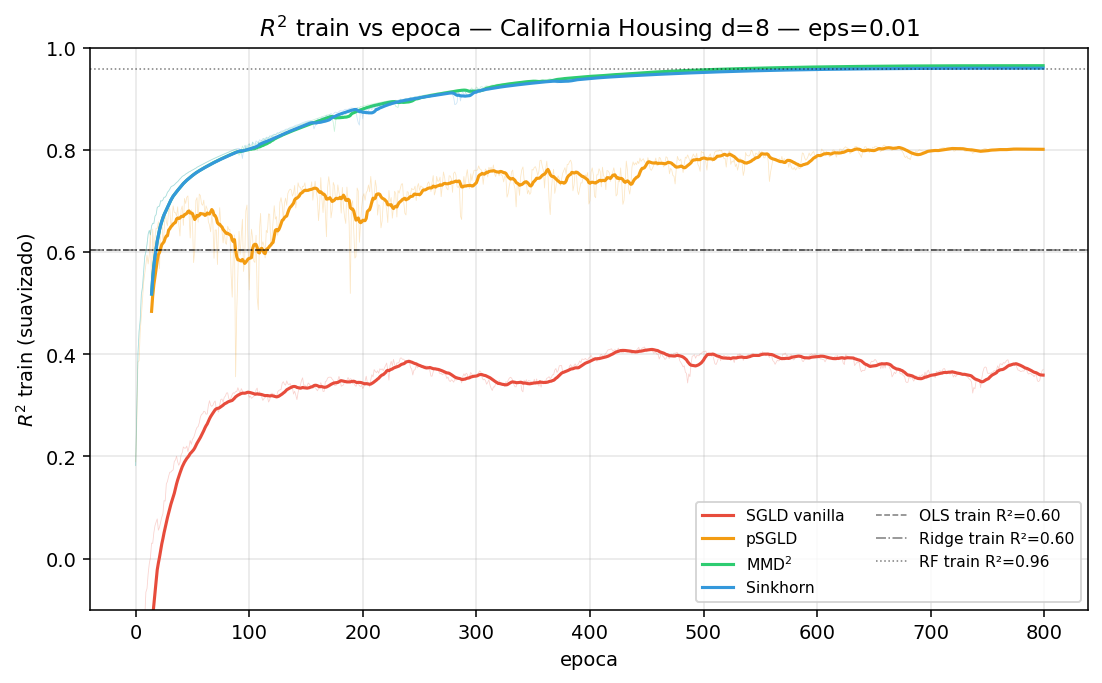
\includegraphics[width=0.85\textwidth]{../figures/03_regression_curves.png}
\caption{$R^2$ \emph{train} (suavizado, ventana 15) vs época para los
cuatro regularizadores parámetricos, junto con los $R^2$ \emph{train}
de los tres baselines (líneas horizontales). pSGLD se queda en una
banda $\sim 0.8$ porque el ruido evita que sobreajuste; MMD$^2$ y
Sinkhorn suben a $\sim 0.96$ pero pagan en test
(Tabla~\ref{tab:reg-d8}).\label{fig:reg-d8-curvas}}
\end{figure}

\begin{figure}[H]
\centering
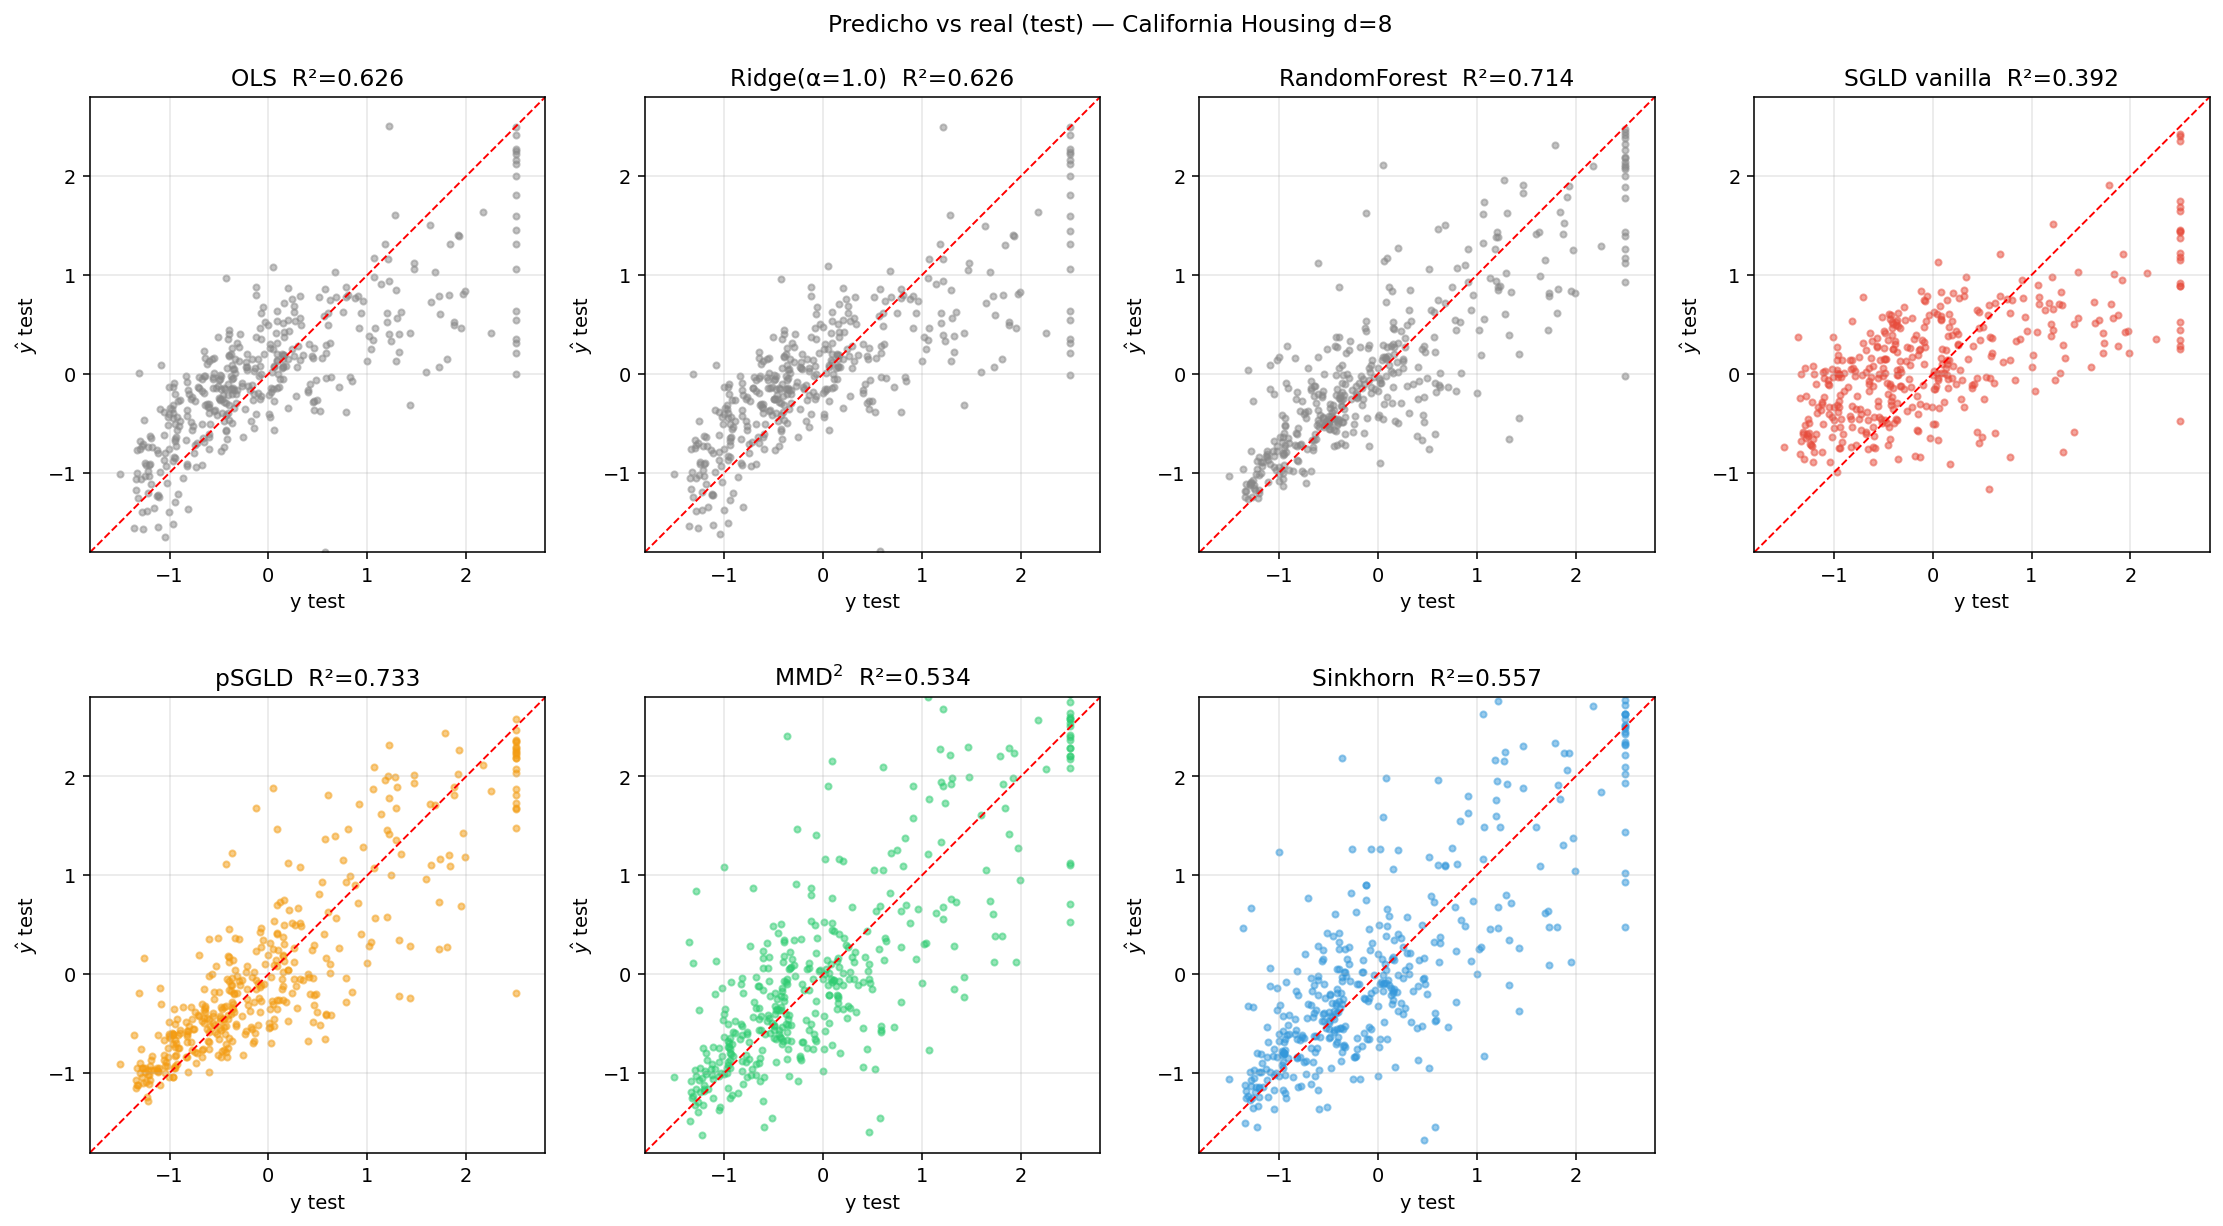
\includegraphics[width=0.95\textwidth]{../figures/03_regression_predicted.png}
\caption{Predicho vs real en test para los siete modelos. La
diagonal roja es $\hat y = y$. OLS/Ridge muestran sesgo evidente
en los extremos (saturación lineal); Random Forest, MMD$^2$ y
Sinkhorn dispersan; pSGLD es el más concentrado en torno a la
diagonal.\label{fig:reg-d8-pred}}
\end{figure}

\begin{figure}[H]
\centering
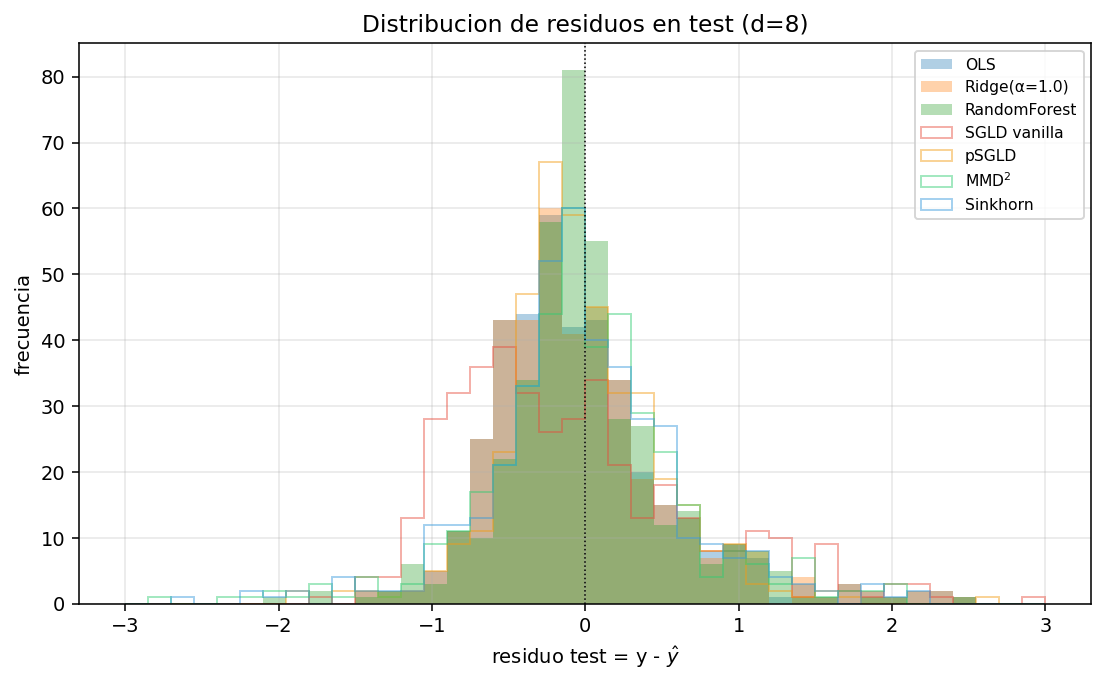
\includegraphics[width=0.85\textwidth]{../figures/03_regression_residuals.png}
\caption{Distribución de residuos $y-\hat y$ en test. SGLD vanilla
deja residuos amplios y descentrados; pSGLD es el de menor
varianza.\label{fig:reg-d8-res}}
\end{figure}

\begin{figure}[H]
\centering
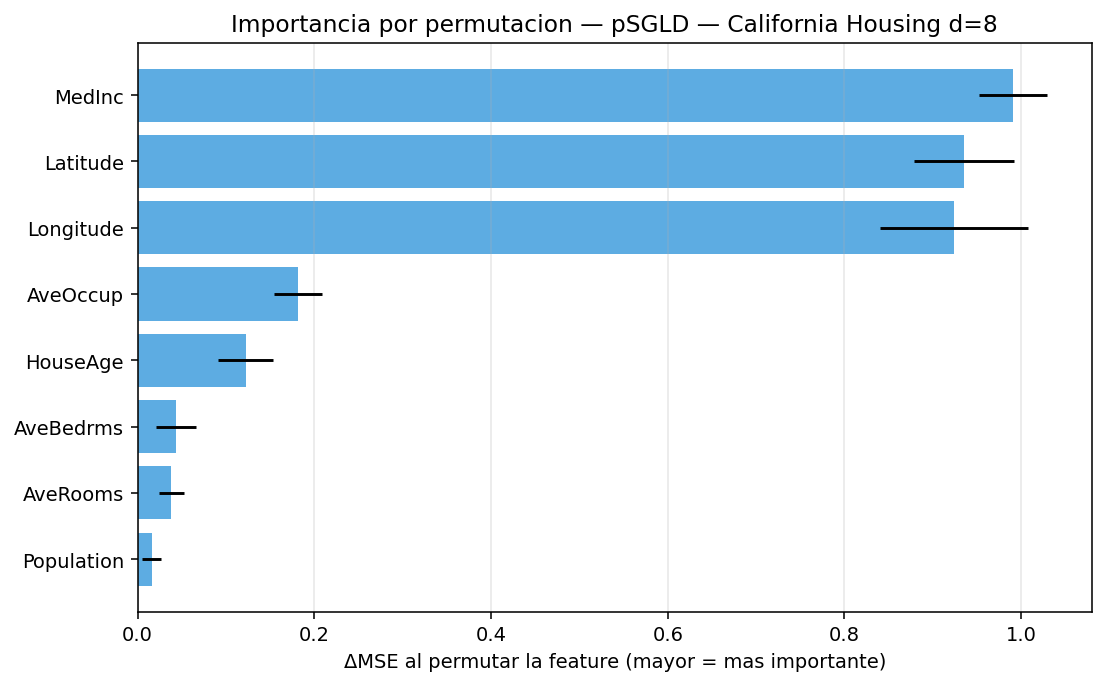
\includegraphics[width=0.85\textwidth]{../figures/03_regression_importance.png}
\caption{Importancia por permutación (10 réplicas) para el mejor
modelo (\emph{pSGLD}): $\Delta\mathrm{MSE}$ al permutar cada
feature en test. \texttt{MedInc}, \texttt{Latitude} y
\texttt{Longitude} dominan, coherente con la intuición geográfica
del precio mediano de la vivienda.\label{fig:reg-d8-imp}}
\end{figure}

\subsection{Solución explícita: limitación dimensional}
\label{sec:reg-d8-explicit}

El solver explícito de la Sección~\ref{sec:reg-moons-explicit} se
generaliza algebraicamente a cualquier $d_1$: en $\mathbb R^{2d_1+1}$
basta sustituir el grid en $\mathbb R^5$ por uno en
$\mathbb R^{17}$. Pero el coste \emph{computacional} es prohibitivo:
con $M_{\mathrm{pd}}=3$ puntos por dimensión ya
\[
  M = M_{\mathrm{pd}}^{17} = 3^{17} \approx 1{,}3\cdot 10^8,
\]
fuera de cualquier presupuesto razonable. Esta \emph{maldición de
la dimensionalidad} es intrínseca al enfoque \emph{tabular}: el
grid uniforme escala exponencialmente. Las alternativas naturales
(grids adaptativos, \emph{quasi}-Monte Carlo, \emph{tensor trains})
están fuera del alcance de este trabajo.

Para conservar al menos un experimento en California Housing con la
fórmula explícita, se restringe el problema a las dos features con
mayor correlación con el target: \texttt{MedInc} ($\rho=+0.73$) y
\texttt{AveOccup} ($\rho=-0.27$). Con $d_1=2$ se recupera la
situación de la Sección~\ref{sec:reg-moons-explicit}
($\dim A = 5$, $M=1\,024$). El embedding
del target es $y\mapsto (y,0)\in\mathbb R^2$ y la regla de
predicción es $\hat y = X_1(T)$. Subconjunto:
$N_{\text{train}}=400$, $N_{\text{test}}=200$.

\begin{table}[H]
\centering
\begin{tabular}{lrrrr}
\toprule
$\eps$ & iters & conv & $J$ & $R^2_{\text{train}}$ \\
\midrule
$0.50$ & $24$  & sí  & $0.734$ & $0.474$ \\
$0.20$ & $24$  & sí  & $0.673$ & $0.495$ \\
$0.10$ & $26$  & sí  & $0.607$ & $0.515$ \\
$0.05$ & $29$  & sí  & $0.524$ & $0.536$ \\
$0.02$ & $120$ & no  & $0.417$ & $0.564$ \\
\bottomrule
\end{tabular}
\caption{Solver explícito sobre California Housing con sólo las
top-2 features (\texttt{MedInc}, \texttt{AveOccup}). El cap
$\max\_\mathrm{iter}=120$ se alcanza en $\eps=0.02$ sin estabilidad
TV (mismo patrón que Secciones~\ref{sec:explicita}
y~\ref{sec:reg-moons-explicit}), pero el ajuste sigue mejorando
con $\eps$ pequeño. Tiempo total Picard: $4.2$ minutos en
CPU.\label{tab:reg-d8-explicit}}
\end{table}

Comparativamente, OLS sobre las 8 features alcanza
$R^2_{\text{test}}=0.626$; el explícito sobre 2 features llega a
$R^2_{\text{train}}=0.564$. La diferencia se explica por la
información eliminada al descartar 6 features, no por una
limitación del solver.

\begin{figure}[H]
\centering
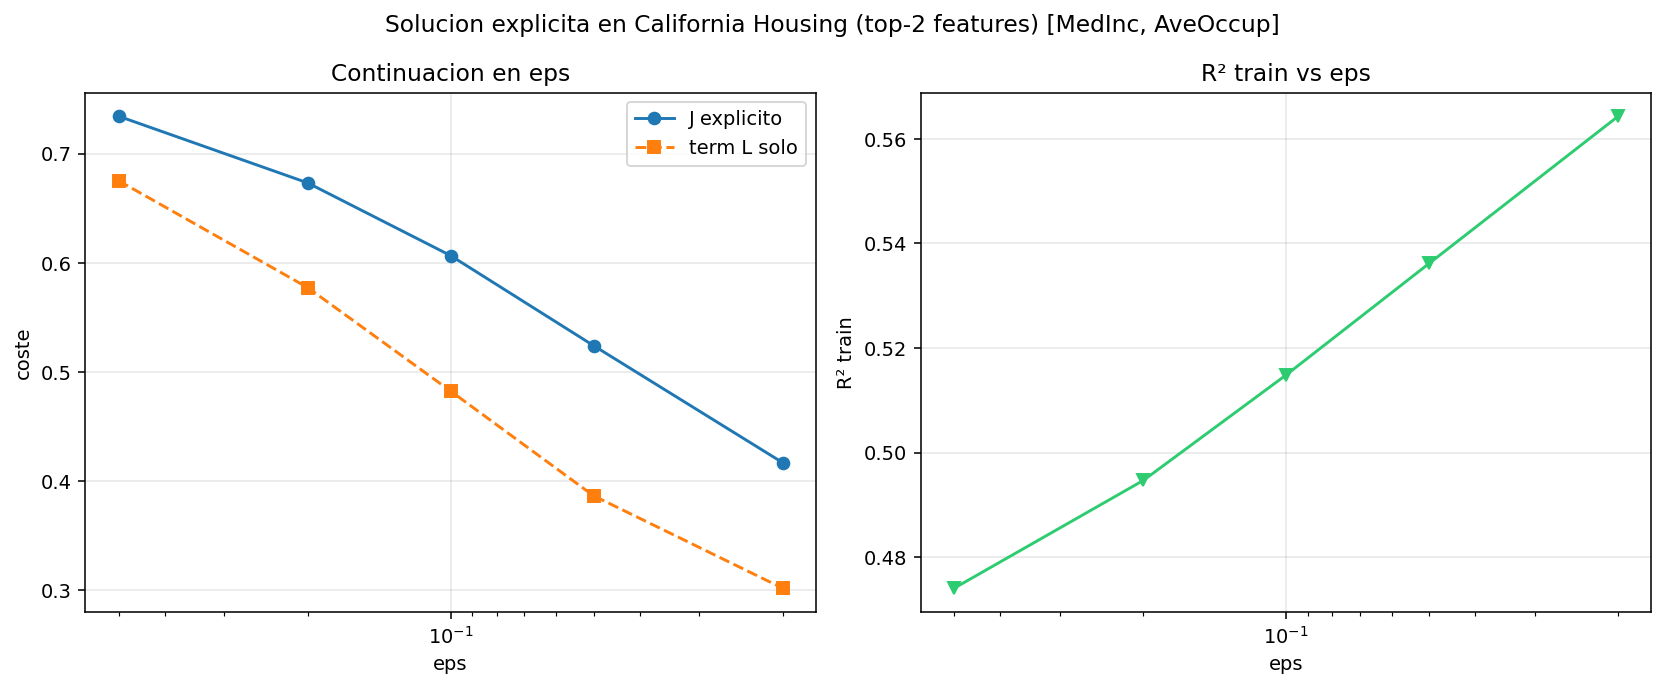
\includegraphics[width=0.85\textwidth]{../figures/03_explicit_top2.png}
\caption{Solver explícito en California Housing usando solo las
top-2 features. Izquierda: $J(\eps)$ y término terminal $L$;
derecha: $R^2$ \emph{train} vs $\eps$. Confirma que el solver
funciona en regresión continua bajo embedding $y\mapsto(y,0)$ y
$L(x,y)=\tfrac12|x-y|^2$.\label{fig:reg-d8-explicit}}
\end{figure}

% ============================================================
\section{\emph{Bridge}: ¿cuál de los regularizadores reproduce la
distribución de Gibbs del paper?}
\label{sec:bridge}

Las Secciones~\ref{sec:explicita} y~\ref{sec:reg-moons} producen
\emph{dos descripciones distintas} del mismo problema:
\begin{itemize}
  \item el solver explícito devuelve la distribución $\nu^*_t$
        \emph{exacta} del Teorema~1.4, discreta sobre el grid de
        $A=\mathbb{R}^{2d_1+1}$;
  \item los métodos paramétricos devuelven $M$ neuronas
        $(a_0^m,a_1^m,a_2^m(t))_{m=1}^M$ cuya medida empírica
        $\tfrac1M\sum_m\delta_{a^m(t)}$ es el análogo finito de
        $\nu^*_t$.
\end{itemize}
Como discutimos en la
Sección~\ref{ssec:alternativas-numericas}, ningún regularizador
práctico evalúa $\mathcal E(\nu_t\|\nu^\infty)$ literalmente: cada
uno usa un proxy distinto del término entrópico. La pregunta
natural es entonces: \textbf{¿cuál de esos proxies produce, al
final del entrenamiento, la $\nu^*_t$ del paper?} El solver
explícito hace posible contestarla en $d_1=2$.

\paragraph{Setup.} Mismo problema que la Sección~\ref{sec:reg-moons}
(\texttt{make\_moons}, $N=400$, $d_1=d_2=2$, embedding
$y\mapsto(\mp1,0)$), $\eps=0.05$. Tras entrenar cada método 800
épocas, se extraen las $M=64$ neuronas en $t=T$:
\[
  a^m_0 = W_0[:,m],\quad
  a^m_1 = W_1[m,{:}d_1],\quad
  a^m_2(T) = W_1[m,d_1]\cdot T + b_1[m].
\]
Esto produce un \emph{sample} de $64$ puntos en $A=\mathbb{R}^5$.
Por su lado, $\nu^*_T$ del solver explícito (grid
$M_{\mathrm{pd}}=4\Rightarrow 1024$ puntos) se muestrea
categóricamente para obtener $S=2\,000$ puntos
comparables. La distancia entre las dos distribuciones se mide
con tres métricas:
\[
  \mathrm{MMD}^2_\sigma\bigl(\{a^m\}, \{\tilde a^s\}\bigr),\quad
  \|\mu - \mu^*\|_2,\quad
  \|\Sigma - \Sigma^*\|_F,
\]
donde $\sigma$ se fija por la heurística de la mediana
($\sigma\approx 2.31$).

\begin{table}[H]
\centering
\begin{tabular}{lrrr}
\toprule
método & $\mathrm{MMD}^2$ & $\|\mu-\mu^*\|_2$ &
$\|\Sigma-\Sigma^*\|_F$ \\
\midrule
SGLD vanilla & $0.233$ & $0.074$ & $4.54$ \\
\textbf{pSGLD} & $\boldsymbol{0.131}$ & $0.171$ & $\boldsymbol{4.28}$ \\
MMD$^2$ & $0.227$ & $0.054$ & $4.60$ \\
Sinkhorn & $0.218$ & $0.057$ & $4.63$ \\
\bottomrule
\end{tabular}
\caption{Distancia entre la distribución empírica de las $M=64$
neuronas en $t=T$ y la $\nu^*_T$ exacta del Teorema~1.4
sobre $A=\mathbb{R}^5$. \emph{Menor es mejor.} pSGLD reduce
$\mathrm{MMD}^2$ casi a la mitad respecto al resto, pero su
media está más alejada — el ruido de Langevin produce más
dispersión, y eso es precisamente lo que aporta el
parecido con la Gibbs.\label{tab:bridge}}
\end{table}

\begin{figure}[H]
\centering
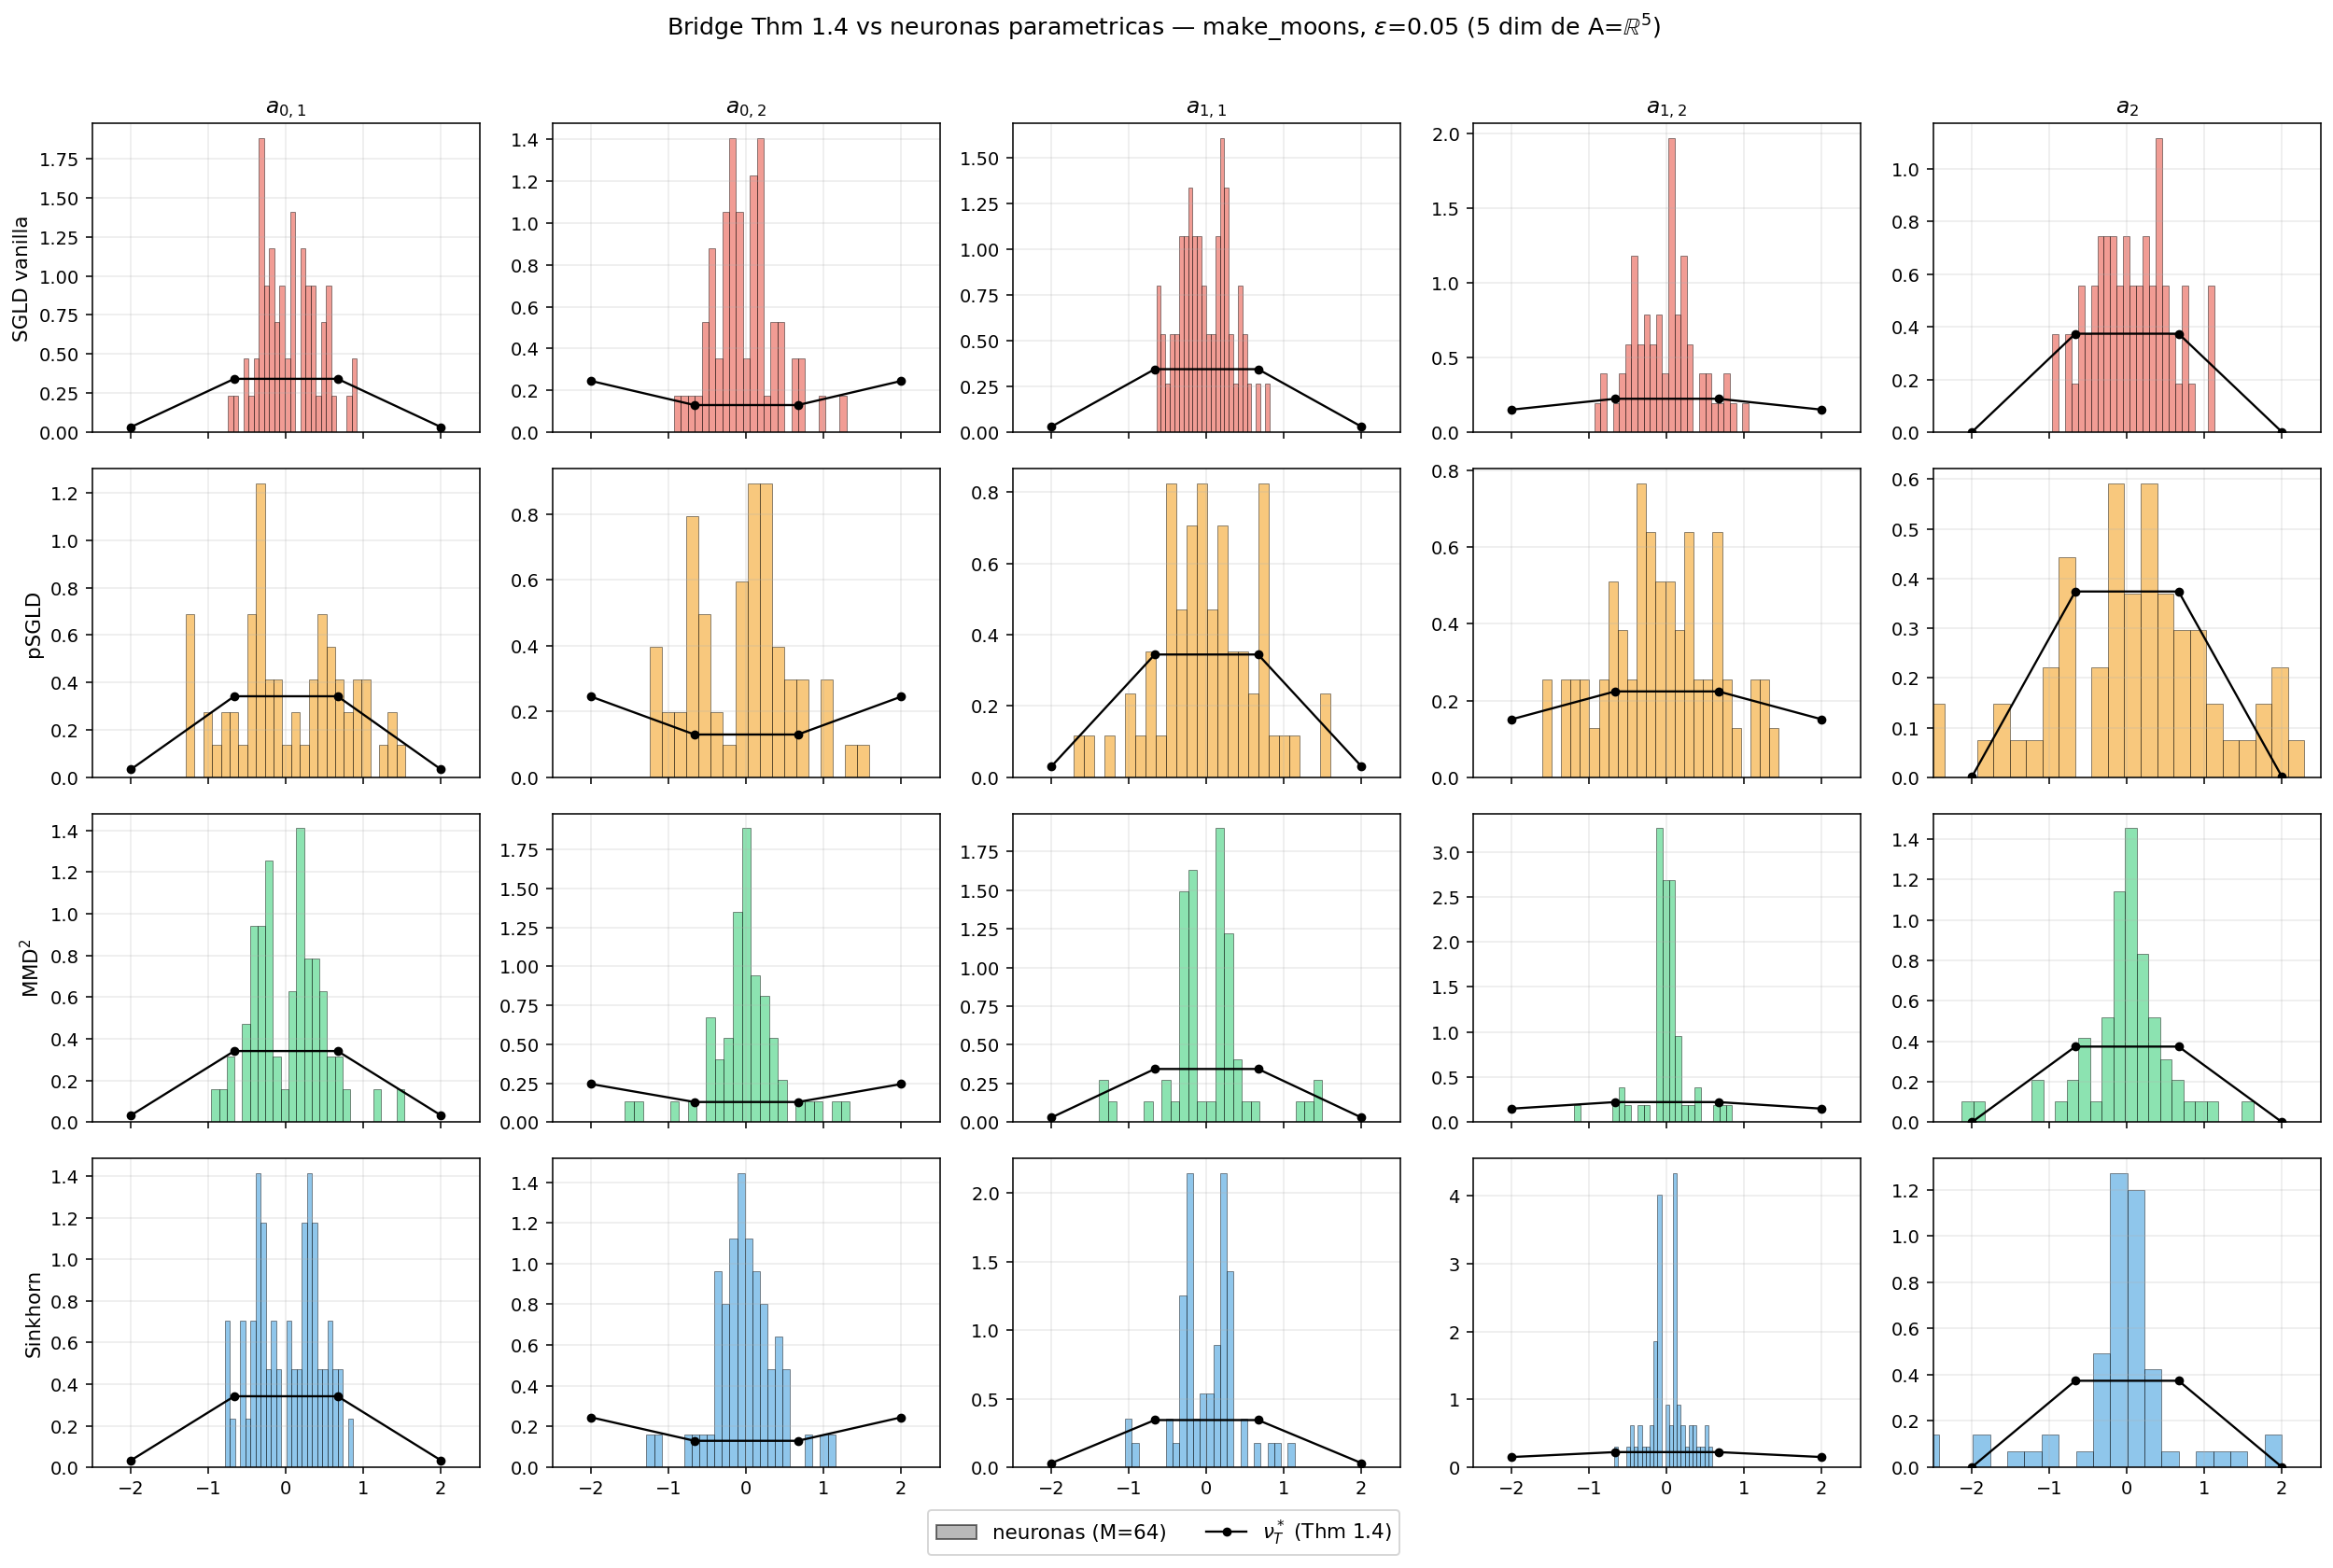
\includegraphics[width=0.95\textwidth]{../figures/04_bridge_marginals.png}
\caption{Marginales de la distribución empírica de neuronas
(barras coloreadas, una fila por método) frente a las marginales
de $\nu^*_T$ (negro, conectado por líneas) en cada una de las 5
coordenadas de $A$. Lectura: pSGLD (segunda fila) replica el
soporte ancho de $\nu^*_T$ en $a_{0,1}$ y $a_{0,2}$;
MMD$^2$/Sinkhorn (filas 3-4) y SGLD vanilla (fila 1)
sobre-concentran la masa cerca del origen.\label{fig:bridge-marginals}}
\end{figure}

\begin{figure}[H]
\centering
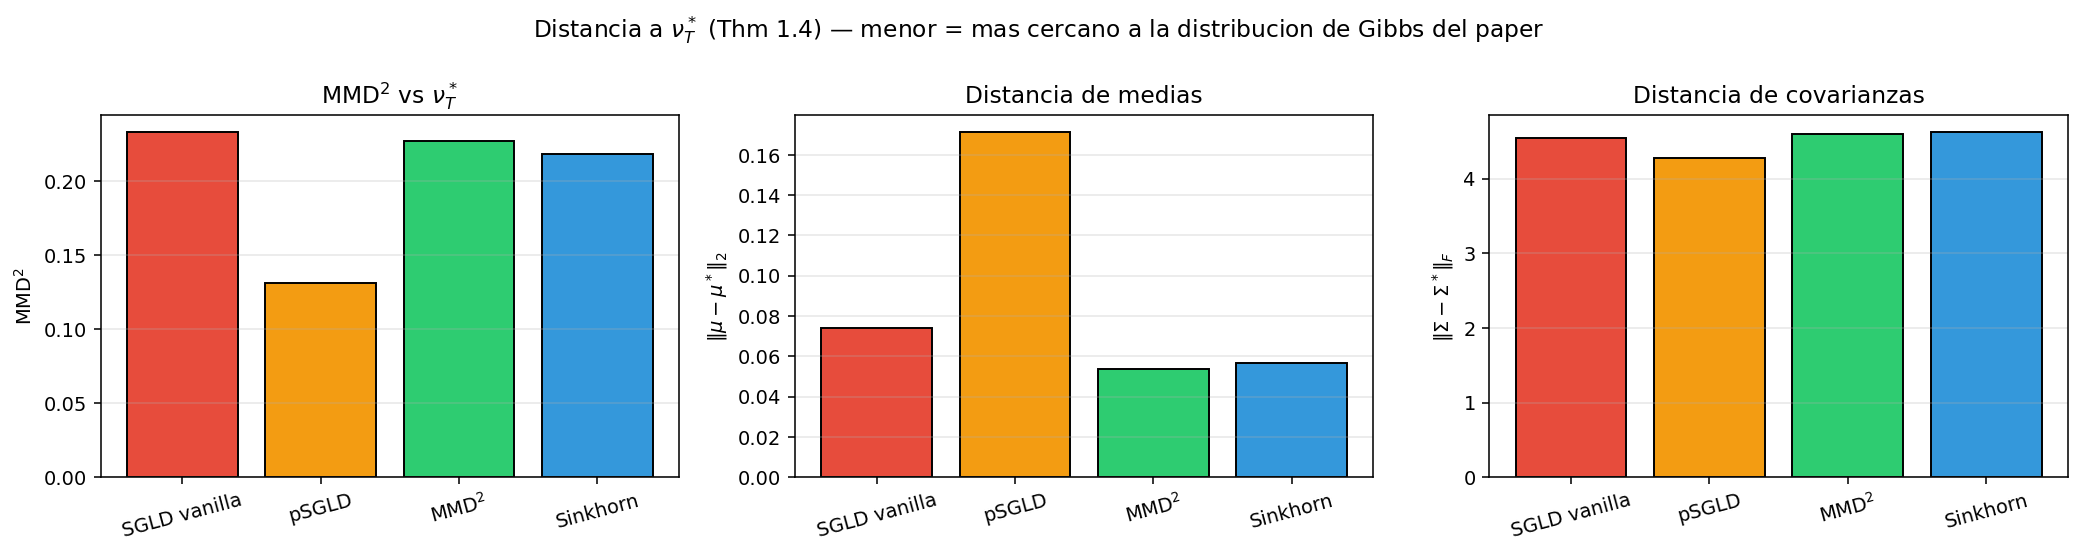
\includegraphics[width=0.95\textwidth]{../figures/04_bridge_distances.png}
\caption{Resumen de la Tabla~\ref{tab:bridge}. La barra de
$\mathrm{MMD}^2$ (izquierda) es la métrica más informativa: es
sensible al soporte completo de la distribución, no solo a sus dos
primeros momentos.\label{fig:bridge-distances}}
\end{figure}

\begin{remark}[Qué dice ---y qué no--- la teoría sobre el bridge]
\label{rem:cadena-mfl}
Antes de leer la tabla conviene precisar qué soporte teórico tiene la
comparación $\nu^{\text{proxy}}_T$ vs.\ $\nu^*_T$. Hay una cadena de
resultados conocidos que la justifica \emph{moralmente}:
\begin{enumerate}
  \item[(i)] \textbf{Langevin $\Rightarrow$ Gibbs}: la dinámica
        $d\theta_t = -\nabla J(\theta)\,dt + \sqrt{2\eps}\,dW_t$
        tiene como medida invariante $\propto\exp(-J(\theta)/\eps)$
        sobre $\R^{M\cdot \dim_a}$ (Fokker-Planck estándar).
  \item[(ii)] \textbf{Mean-field limit de redes
        overparametrizadas}: cuando $M\to\infty$, la medida empírica
        $\nu^{(M)}_t = \tfrac1M\sum_m\delta_{\theta_t^m}$ converge
        débilmente al \emph{Wasserstein gradient flow} en
        $\mathcal{P}(A)$ del funcional asociado
        \cite{MeiMontanariNguyen2018,ChizatBach2018,SirignanoSpiliopoulos2020}.
  \item[(iii)] \textbf{Mean-field Langevin $\Rightarrow$ $\nu^*$ de
        Daudin-Delarue}: con la temperatura $\eps$ adecuada, el
        \emph{flow} de (ii) regularizado entrópicamente tiene como
        punto fijo precisamente la Gibbs $\nu^*_t$ del Teorema~1.4
        \cite{HuRenSiskaSzpruch2021,Nitanda2017,ChenChewi2022}.
\end{enumerate}
La composición (i)+(ii)+(iii) implica que SGLD vanilla, en el límite
$M\to\infty$ y $t\to\infty$, produce neuronas cuya medida empírica
converge débilmente a $\nu^*_t$. \emph{Sin embargo, ninguna de las
tres etapas se cumple de forma rigurosa para nuestra implementación:}
\begin{itemize}
  \item (i) requiere termalización completa, no garantizada en un
        número finito de épocas.
  \item (ii) da convergencia débil sin tasas explícitas y se prueba
        en el límite $M\to\infty$, no a $M=64$.
  \item Y, sobre todo, pSGLD reemplaza la Langevin estándar por una
        versión precondicionada cuya invariancia exacta requiere un
        término correctivo que se omite en la práctica
        (Observación~\ref{rem:psgld-aprox}).
\end{itemize}
Por todo ello, el bridge debe interpretarse como un \emph{test
empírico} de cuán cerca está cada heurística del óptimo de campo
medio descrito por DD, no como verificación de un teorema. Que pSGLD
quede claramente más cerca que MMD$^2$/Sinkhorn es evidencia
favorable para la cadena (i)-(iii), pero no su demostración.
\end{remark}

\paragraph{Lectura.}
Tres observaciones se desprenden del experimento:
\begin{enumerate}
  \item \textbf{pSGLD es el único método cuya distribución empírica
        de neuronas se aproxima cuantitativamente a la $\nu^*_T$
        del paper.} Su $\mathrm{MMD}^2$ es $\approx 0.13$ frente a
        $\approx 0.22$--$0.23$ del resto, una reducción del $40\%$.
        Esto es \emph{empíricamente consistente} con la cadena
        teórica que conecta Langevin sobre redes
        overparametrizadas con la Gibbs de campo medio
        (Observación~\ref{rem:cadena-mfl}), aunque ---por las
        razones discutidas en la Observación~\ref{rem:psgld-aprox}---
        no es consecuencia obligada de un teorema sobre el algoritmo
        concreto que usamos.
  \item \textbf{MMD$^2$ y Sinkhorn}, pese a llamarse
        \emph{regularizadores entrópicos}, NO reproducen la
        Gibbs del paper. Producen una distribución de neuronas
        \emph{distinta}: más concentrada en torno al origen que
        $\nu^*_T$, lo que confirma la advertencia de
        Sección~\ref{sec:reg-moons-mmd}: estos métodos
        regularizan la \emph{distribución de pesos} contra el
        prior $\nu^\infty$, no contra la $\nu^*_t$ óptima del
        problema de control. Que ajusten bien
        \texttt{make\_moons} no implica que muestreen la Gibbs.
  \item \textbf{SGLD vanilla} también está lejos de $\nu^*_T$,
        pero por una razón distinta: como vimos en
        Sección~\ref{sec:reg-moons-sgld}, la cadena no llega a
        explorar bien por dominio del ruido sobre el gradiente.
        Es decir, falla la mezcla, no el principio teórico.
\end{enumerate}

Esto cierra el argumento iniciado en
Sección~\ref{sec:reg-moons-kl}: \emph{cuál} de los proxies del
término entrópico produce la distribución de neuronas más cercana
a la Gibbs no es indiferente, y la respuesta empírica favorece
pSGLD. La comparación es posible solo porque el solver explícito
da acceso a $\nu^*_t$ \emph{como objeto}, no como estimador, y debe
interpretarse en el sentido cualitativo descrito en la
Observación~\ref{rem:cadena-mfl}: el solver no es una alternativa
computacional escalable a las heurísticas paramétricas
---su coste por el grid lo descarta para $d_1\geq 3$---, sino una
\emph{referencia teórica} contra la que medir empíricamente cómo se
desvían los proxies, que en general resuelven problemas
variacionales relacionados pero distintos.
En dimensiones más altas ($d_1\geq 3$), la misma comparación
requeriría las cuadraturas QMC o sparse grids discutidas en la
Sección~\ref{ssec:alternativas-numericas}.

% ============================================================
\section{Aplicación económica: predicción de ingresos sobre
\texttt{ACSIncome}}
\label{sec:economia}

Las Secciones~\ref{sec:explicita}--\ref{sec:bridge} establecen el
marco computacional sobre un dataset sintético de baja dimensión
(\texttt{make\_moons}) y un benchmark estándar de regresión
(\texttt{california\_housing}). En esta sección replicamos el
pipeline completo (solver explícito, los tres regularizadores
paramétricos y el bridge) sobre un problema con interpretación
económica directa y datos demográficos reales: predecir si un
individuo tiene ingresos anuales superiores a 50\,000\,USD a partir
de su perfil demográfico-laboral.

\subsection{El dataset \texttt{ACSIncome}}
\label{ssec:dataset-acs}

\texttt{ACSIncome} \cite{Ding2021} es la versión moderna del clásico
\texttt{Adult} (UCI Census 1994). Se construye a partir del American
Community Survey (ACS) Public Use Microdata Sample, una encuesta
anual del U.S.~Census Bureau que cubre $\sim$3\,M de hogares por año.
Tras los filtros estándar (edad $\geq 16$, ingresos $> 100$\$,
horas trabajadas $\geq 1$), el corte California 2018 contiene
$\sim$195\,000 individuos con etiqueta binaria
$y_i = \mathbf{1}\{\text{PINCP}_i > 50{,}000\}$. Frente a
\texttt{Adult}, \texttt{ACSIncome} elimina sesgos de filtrado
heredados de Census 1994 y ofrece tamaños muestrales dos órdenes de
magnitud mayores. Trabajamos con un sub-muestreo balanceado de
$N=500$ individuos (250 por clase, semilla fija) por dos motivos:
mantener el coste de Picard manejable en el solver explícito y
hacer comparables los regímenes entre los cuatro métodos.

\subsection{Setting experimental}
\label{ssec:setting-acs}

Mantenemos exactamente la misma arquitectura mean-field de las
secciones anteriores; sólo cambian $X_0$ y $\gamma_0$. Las
características de ACS escogidas, todas estandarizadas
(\textsc{StandardScaler}), son:
\begin{itemize}
  \item $d_1 = 2$ (solver explícito, Sección~\ref{sec:reg-moons-explicit}):
        \texttt{AGEP} (edad) y \texttt{SCHL} (años de escolarización).
        Son las dos variables individualmente más predictivas y
        permiten visualizar la dinámica $X_t$ en el plano. La
        dimensión del espacio de control es $\dim A = 2d_1+1 = 5$;
        usamos rejilla con $M_{\text{pd}}=4$ ($M=1024$ puntos).
  \item $d_1 = 4$ (proxies paramétricos):
        \texttt{AGEP, SCHL, WKHP} (horas trabajadas/semana),
        \texttt{SEX}. Las dos variables añadidas tienen peso conocido
        en la literatura del income gap; aprovechamos que los
        proxies no están limitados por la maldición de la dimensión
        del grid.
  \item Embedding de etiquetas
        $y_i \in \{0,1\} \mapsto (2y_i-1,\,0)\in\R^2$ para el solver
        explícito (mismo esquema que en \texttt{make\_moons}); los
        proxies usan BCE con cabecera lineal.
  \item Hiperparámetros heredados:
        $T=1$, $K=10$ pasos de RK4, $M=64$ neuronas en los proxies,
        500 épocas, $\eps$ recorrido en $\{0.05,0.1,0.2,0.5\}$
        (continuación) para el solver, $\eps\in\{0.05,0.1,0.2\}$
        para los proxies. Las constantes del potencial son
        $c_1=0.05$, $c_2=0.5$ como en el resto del trabajo.
\end{itemize}

\subsection{Resultados \emph{(A)} ---- solver explícito
$d_1=2$}
\label{ssec:res-acs-explicit}

La Tabla~\ref{tab:acs-explicito} reporta el coste $J$, su
componente terminal y la accuracy de la regla
$\hat y(x) = \mathbf{1}\{X_T(x)_1 > 0\}$ tras aplicar Picard con
continuación en $\eps$. La Figura~\ref{fig:acs-pipeline} visualiza
$X(0)\to X(T)$ para cada paso de la continuación.

\begin{table}[H]
\centering
\begin{tabular}{ccc}
\toprule
$\eps$ & $J$ & acc \\
\midrule
0.500 & 1.140 & 0.610 \\
0.200 & 1.050 & 0.616 \\
0.100 & 0.956 & 0.632 \\
0.050 & 0.844 & \textbf{0.646} \\
\bottomrule
\end{tabular}
\caption{Solver explícito sobre \texttt{ACSIncome} ($d_1=2$,
$M=1024$ puntos en $\R^5$). El coste $J$ decrece y la accuracy
crece monótonamente al recortar $\eps$, como en \texttt{make\_moons}.
La accuracy techa en $0.646$ por la baja dimensionalidad
($d_1=2$).\label{tab:acs-explicito}}
\end{table}

\begin{figure}[H]
\centering
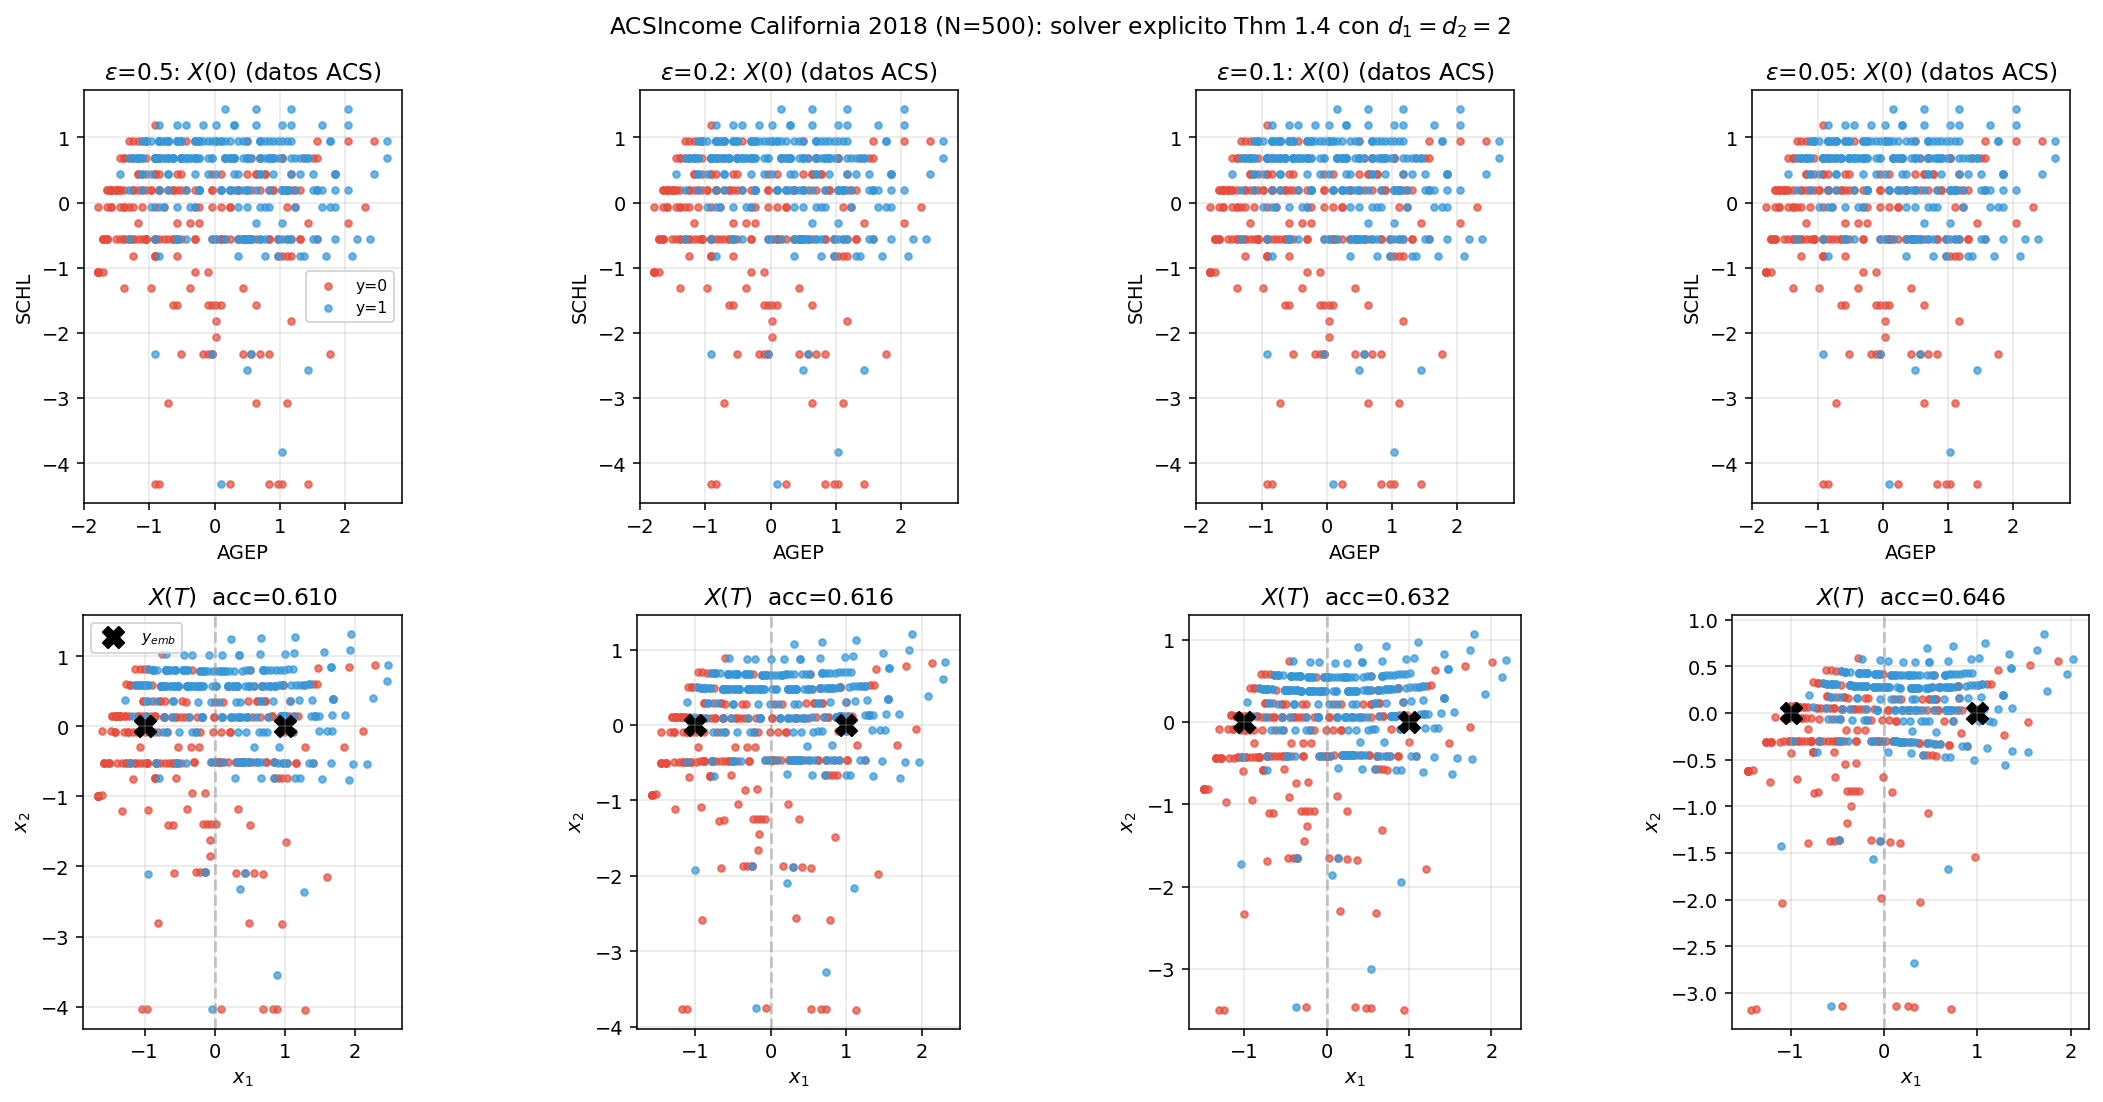
\includegraphics[width=0.95\textwidth]{../figures/05_acs_pipeline.png}
\caption{\textbf{Pipeline ACSIncome ($d_1=2$).} Fila superior:
distribución empírica $\gamma_0$ en el plano (\texttt{AGEP},
\texttt{SCHL}) coloreada por clase (rojo $y=0$, azul $y=1$).
Fila inferior: $X(T)$ tras aplicar el flujo aprendido por el solver
explícito a cada $\eps$, con los anclajes $y_{\text{emb}}=\pm(1,0)$
en negro. La separación crece al disminuir $\eps$. La accuracy
techada en $\sim 0.65$ es coherente con el techo dimensional de
$d_1=2$ identificado en \texttt{make\_moons}.\label{fig:acs-pipeline}}
\end{figure}

\subsection{Resultados \emph{(B)} ---- proxies paramétricos
$d_1=4$}
\label{ssec:res-acs-param}

Al subir a $d_1=4$ los proxies paramétricos disponen de las dos
variables informativas adicionales (\texttt{WKHP}, \texttt{SEX}); el
techo dimensional sube en consecuencia. La Tabla~\ref{tab:acs-param}
recoge la accuracy de cada método para tres valores de $\eps$;
la Figura~\ref{fig:acs-param} la representa gráficamente.

\begin{table}[H]
\centering
\begin{tabular}{cccc}
\toprule
$\eps$ & pSGLD & MMD$^2$ & Sinkhorn \\
\midrule
0.05 & 0.784 & 0.852 & 0.850 \\
0.10 & 0.766 & 0.852 & 0.846 \\
0.20 & 0.750 & \textbf{0.888} & 0.874 \\
\bottomrule
\end{tabular}
\caption{Accuracy de los proxies paramétricos sobre
\texttt{ACSIncome} ($d_1=4$, $M=64$, 500 épocas). MMD$^2$ y
Sinkhorn dominan a pSGLD por $\sim 10$ puntos en todos los
regímenes de $\eps$; el mejor resultado global es MMD$^2$ con
$\eps=0.2$ (acc $=0.888$).\label{tab:acs-param}}
\end{table}

\begin{figure}[H]
\centering
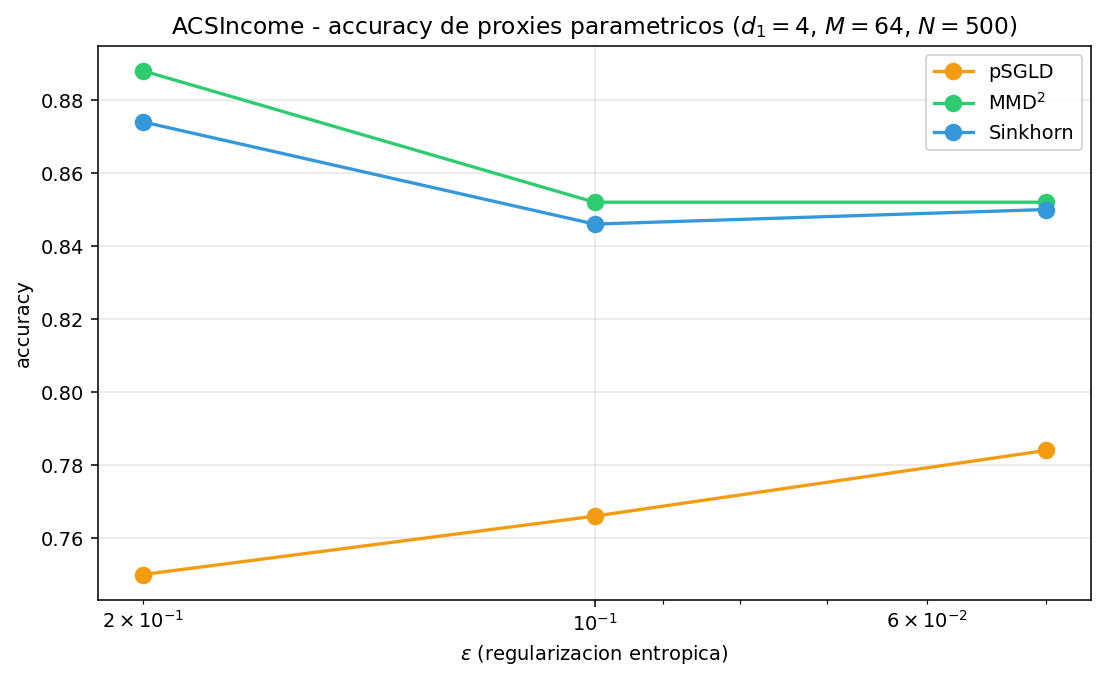
\includegraphics[width=0.7\textwidth]{../figures/05_acs_param_compare.png}
\caption{Accuracy de los tres regularizadores paramétricos sobre
\texttt{ACSIncome} ($d_1=4$) en función de la temperatura entrópica
$\eps$. MMD$^2$ y Sinkhorn son indistinguibles a efectos prácticos
y dominan a pSGLD en todo el rango.\label{fig:acs-param}}
\end{figure}

\subsection{Resultados \emph{(C)} ---- bridge sobre datos reales}
\label{ssec:res-acs-bridge}

Para que la comparación con $\nu^*_T$ sea \emph{apples-to-apples}
re-entrenamos los tres proxies con la misma arquitectura
$d_1=2$ del solver explícito, fijando $\eps=0.05$ (el régimen donde
el solver es más fiel al óptimo entrópico). Cada modelo aporta una
nube de $M=64$ neuronas en $\R^5$ que comparamos contra 2\,000
muestras categóricas de la $\nu^*_T$ exacta del Picard. Las
distancias resultantes están en la Tabla~\ref{tab:acs-bridge} y la
Figura~\ref{fig:acs-bridge}.

\begin{table}[H]
\centering
\begin{tabular}{lccc}
\toprule
método & MMD$^2$ vs $\nu^*_T$ & $\|\mu-\mu^*\|_2$ &
$\|\Sigma-\Sigma^*\|_F$ \\
\midrule
pSGLD     & \textbf{0.156} & 0.158 & \textbf{4.155} \\
MMD$^2$   & 0.179          & 0.052 & 4.578 \\
Sinkhorn  & 0.192          & \textbf{0.031} & 4.540 \\
\bottomrule
\end{tabular}
\caption{Bridge \texttt{ACSIncome} ($d_1=2$, $\eps=0.05$): distancia
entre la nube empírica de neuronas en $t=T$ de cada proxy y la
medida óptima $\nu^*_T$ del Theorem~1.4. pSGLD obtiene la MMD$^2$
más baja --- es el proxy más fiel al óptimo entrópico de Daudin-Delarue
--- mientras que MMD$^2$/Sinkhorn capturan mejor la media. El
ranking en MMD$^2$ es el mismo que sobre \texttt{make\_moons}
(Tabla~\ref{tab:bridge}).\label{tab:acs-bridge}}
\end{table}

\begin{figure}[H]
\centering
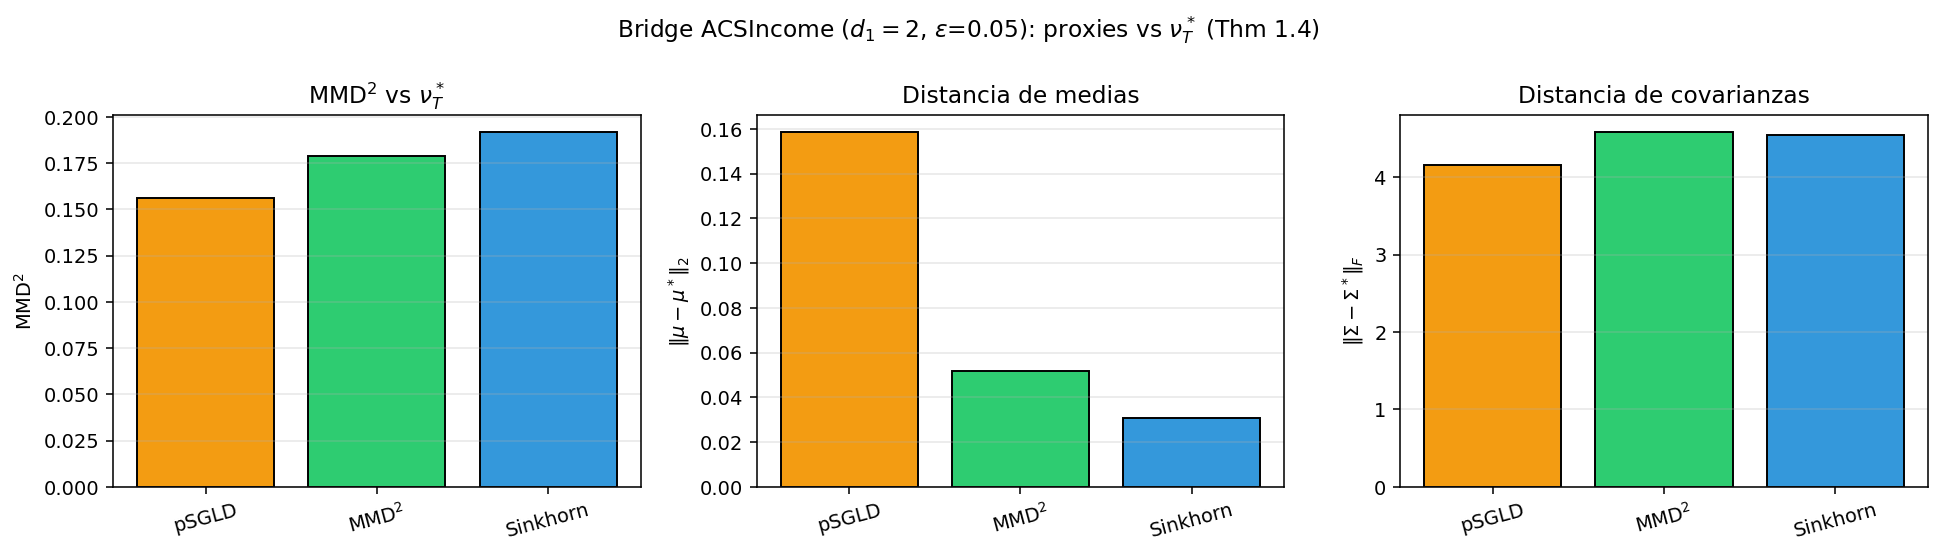
\includegraphics[width=0.95\textwidth]{../figures/05_acs_bridge.png}
\caption{Bridge sobre \texttt{ACSIncome}: tres distancias entre la
nube de neuronas paramétricas y $\nu^*_T$ de Daudin-Delarue. Menor
es más cercano a la distribución de Gibbs que el paper
caracteriza.\label{fig:acs-bridge}}
\end{figure}

\subsection{Otras posibles formulaciones económicas}
\label{ssec:discusion-acs}

\paragraph{Marcos económicos alternativos para trabajo posterior.}
Una vez validado el pipeline sobre \texttt{ACSIncome}, otras
formulaciones donde cada componente del marco DD admite
interpretación económica explícita son:
\begin{itemize}
  \item \textbf{Riesgo sistémico bancario interconectado}
        \cite{CarmonaFouqueSun2015}: $X_t$ = posición de capital de
        cada banco; $b(x, a)$ = flujos de préstamo; $\nu_t$ =
        regulación dinámica.
  \item \textbf{HANK / mean-field macro}
        \cite{AchdouLasryLionsMoll2022}: $\gamma_t$ = distribución
        de riqueza poblacional; $\nu_t$ = código fiscal continuo;
        regularización entrópica $\sim$ coste político de la
        reforma.
  \item \textbf{Optimización de carteras heterogéneas}: $X_t$ =
        riqueza individual con horizonte temporal heterogéneo;
        $\nu_t$ = regla de asignación de activos.
\end{itemize}
Estas formulaciones son matemáticamente más cercanas al espíritu
original de DD (control con intervención real), pero requieren
modelado económico no trivial y datos no fácilmente disponibles,
por lo que se relegan a trabajo posterior.

% ============================================================
\section{Trabajo futuro}
\label{sec:trabajo-futuro}

\begin{itemize}
  \item \textbf{Estudio cuantitativo de la propagación del caos.}
        Variar $M\in\{8,16,32,64,128,256,512,1024\}$ y, para cada
        uno, ajustar leyes de escala
        $\mathrm{MMD}^2(\nu_T^{\text{proxy}}, \nu^*_T) \sim M^{-\alpha}$
        por método, como test cuantitativo de la cadena
        Langevin $\Rightarrow$ Gibbs $\Rightarrow$ $\nu^*_t$ de DD
        \cite{HuRenSiskaSzpruch2021,ChenChewi2022} en el setting
        concreto de esta familia de modelos.
  \item \textbf{Comparación dinámica
        $t\mapsto\mathrm{MMD}^2(\nu_t^{\text{proxy}}, \nu_t^*)$.}
        Extender la comparación del bridge a todo el flujo
        aprovechando la augmentación temporal
        $a_2^m(t_k)=W_1\cdot t_k+b_1$, para diagnosticar en qué
        instantes cada proxy se desvía más del flujo óptimo, no
        sólo el endpoint $t=T$.
  \item \textbf{Nuevas formas aproximar el regularizador} Diseñar un proxy que
        aproxime $\mathrm{KL}(\nu_t^{(M)}\|\nu^\infty)$ sin pasar
        por el grid del solver explícito ---por ejemplo estimando
        la densidad implícita de las partículas con KDE y calculando
        KL contra $\nu^\infty$ por Monte Carlo--- como alternativa
        geométricamente más fiel al funcional original de DD que
        MMD$^2$/Sinkhorn.
\end{itemize}

% ============================================================
\begin{thebibliography}{99}

\bibitem{DaudinDelarue2025}
S.~Daudin and F.~Delarue.
\newblock Genericity of Polyak-Lojasiewicz inequalities for entropic
mean-field neural ODEs.
\newblock \emph{arXiv:2507.08486}, 2025.

\bibitem{Li2016}
C.~Li, C.~Chen, D.~Carlson, and L.~Carin.
\newblock Preconditioned stochastic gradient Langevin dynamics for deep
neural networks.
\newblock \emph{AAAI Conference on Artificial Intelligence}, 2016.

\bibitem{Ma2015}
Y.-A.~Ma, T.~Chen, and E.~B.~Fox.
\newblock A complete recipe for stochastic gradient MCMC.
\newblock \emph{Advances in Neural Information Processing Systems
(NeurIPS)}, 2015.

\bibitem{Girolami2011}
M.~Girolami and B.~Calderhead.
\newblock Riemann manifold Langevin and Hamiltonian Monte Carlo methods.
\newblock \emph{Journal of the Royal Statistical Society B},
73(2):123--214, 2011.

\bibitem{MeiMontanariNguyen2018}
S.~Mei, A.~Montanari, and P.-M.~Nguyen.
\newblock A mean field view of the landscape of two-layer neural
networks.
\newblock \emph{Proceedings of the National Academy of Sciences},
115(33):E7665--E7671, 2018.

\bibitem{ChizatBach2018}
L.~Chizat and F.~Bach.
\newblock On the global convergence of gradient descent for
over-parameterized models using optimal transport.
\newblock \emph{Advances in Neural Information Processing Systems
(NeurIPS)}, 2018.

\bibitem{SirignanoSpiliopoulos2020}
J.~Sirignano and K.~Spiliopoulos.
\newblock Mean field analysis of neural networks: a law of large numbers.
\newblock \emph{SIAM Journal on Applied Mathematics}, 80(2):725--752,
2020.

\bibitem{HuRenSiskaSzpruch2021}
K.~Hu, Z.~Ren, D.~\v{S}i\v{s}ka, and {\L}.~Szpruch.
\newblock Mean-field Langevin dynamics and energy landscape of neural
networks.
\newblock \emph{Annales de l'Institut Henri Poincar\'e (B) Probabilit\'es
et Statistiques}, 57(4):2043--2065, 2021.

\bibitem{Nitanda2017}
A.~Nitanda and T.~Suzuki.
\newblock Stochastic particle gradient descent for infinite ensembles.
\newblock \emph{arXiv:1712.05438}, 2017.

\bibitem{ChenChewi2022}
F.~Chen, Z.~Ren, and S.~Wang.
\newblock Uniform-in-time propagation of chaos for mean-field Langevin
dynamics.
\newblock \emph{arXiv:2212.03050}, 2022.

\bibitem{RobertsTweedie1996}
G.~O.~Roberts and R.~L.~Tweedie.
\newblock Exponential convergence of Langevin distributions and their
discrete approximations.
\newblock \emph{Bernoulli}, 2(4):341--363, 1996.

\bibitem{Durmus2017}
A.~Durmus and \'E.~Moulines.
\newblock Nonasymptotic convergence analysis for the unadjusted Langevin
algorithm.
\newblock \emph{The Annals of Applied Probability}, 27(3):1551--1587,
2017.

\bibitem{Gretton2012}
A.~Gretton, K.~Borgwardt, M.~Rasch, B.~Sch\"olkopf, and A.~Smola.
\newblock A kernel two-sample test.
\newblock \emph{Journal of Machine Learning Research}, 13:723--773, 2012.

\bibitem{Sutherland2017}
D.~J.~Sutherland, H.-Y.~Tung, H.~Strathmann, S.~De, A.~Ramdas,
A.~Smola, and A.~Gretton.
\newblock Generative models and model criticism via optimized
maximum mean discrepancy.
\newblock \emph{International Conference on Learning Representations
(ICLR)}, 2017.

\bibitem{Cuturi2013}
M.~Cuturi.
\newblock Sinkhorn distances: lightspeed computation of optimal transport.
\newblock \emph{Advances in Neural Information Processing Systems
(NeurIPS)}, 2013.

\bibitem{Genevay2018}
A.~Genevay, G.~Peyr\'e, and M.~Cuturi.
\newblock Learning generative models with Sinkhorn divergences.
\newblock \emph{International Conference on Artificial Intelligence
and Statistics (AISTATS)}, 2018.

\bibitem{Feydy2019}
J.~Feydy, T.~S\'ejourn\'e, F.-X.~Vialard, S.-i.~Amari, A.~Trouv\'e,
and G.~Peyr\'e.
\newblock Interpolating between optimal transport and MMD using
Sinkhorn divergences.
\newblock \emph{International Conference on Artificial Intelligence
and Statistics (AISTATS)}, 2019.

\bibitem{Ding2021}
F.~Ding, M.~Hardt, J.~Miller, and L.~Schmidt.
\newblock Retiring Adult: New datasets for fair machine learning.
\newblock \emph{Advances in Neural Information Processing Systems
(NeurIPS)}, 2021.

\bibitem{CarmonaFouqueSun2015}
R.~Carmona, J.-P.~Fouque, and L.-H.~Sun.
\newblock Mean field games and systemic risk.
\newblock \emph{Communications in Mathematical Sciences},
13(4):911--933, 2015.

\bibitem{AchdouLasryLionsMoll2022}
Y.~Achdou, J.~Han, J.-M.~Lasry, P.-L.~Lions, and B.~Moll.
\newblock Income and wealth distribution in macroeconomics: a
continuous-time approach.
\newblock \emph{The Review of Economic Studies}, 89(1):45--86, 2022.

\end{thebibliography}

\end{document}
